%%%%%%%%%%%%%%%%%%%%%%%%%%%%%%%%%%%%%%%%%
% Masters/Doctoral Thesis 
% LaTeX Template
% Version 2.5 (27/8/17)
%
% This template was downloaded from:
% http://www.LaTeXTemplates.com
%
% Version 2.x major modifications by:
% Vel (vel@latextemplates.com)
%
% This template is based on a template by:
% Steve Gunn (http://users.ecs.soton.ac.uk/srg/softwaretools/document/templates/)
% Sunil Patel (http://www.sunilpatel.co.uk/thesis-template/)
%
% Template license:
% CC BY-NC-SA 3.0 (http://creativecommons.org/licenses/by-nc-sa/3.0/)
%
%%%%%%%%%%%%%%%%%%%%%%%%%%%%%%%%%%%%%%%%%

%----------------------------------------------------------------------------------------
%	PACKAGES AND OTHER DOCUMENT CONFIGURATIONS
%----------------------------------------------------------------------------------------

\documentclass[
12pt, % The default document font size, options: 10pt, 11pt, 12pt
%oneside, % Two side (alternating margins) for binding by default, uncomment to switch to one side
english, % ngerman for German
onehalfspacing,  % Single line spacing, alternatives: singlespacing, onehalfspacing or doublespacing
%draft, % Uncomment to enable draft mode (no pictures, no links, overfull hboxes indicated)
nolistspacing, % If the document is onehalfspacing or doublespacing, uncomment this to set spacing in lists to single
liststotoc, % Uncomment to add the list of figures/tables/etc to the table of contents
%toctotoc, % Uncomment to add the main table of contents to the table of contents
%parskip, % Uncomment to add space between paragraphs
%nohyperref, % Uncomment to not load the hyperref package
headsepline, % Uncomment to get a line under the header
%chapterinoneline, % Uncomment to place the chapter title next to the number on one line
%consistentlayout, % Uncomment to change the layout of the declaration, abstract and acknowledgements pages to match the default layout
]{MastersDoctoralThesis} % The class file specifying the document structure

\usepackage[utf8]{inputenc} % Required for inputting international characters
\usepackage{pdfpages}
\usepackage[T1]{fontenc} % Output font encoding for international characters
\usepackage{amsmath}
\usepackage{mathpazo} % Use the Palatino font by default
\usepackage{float}
\usepackage[backend=bibtex,style=numeric,sorting=none,natbib=true,backref=true,url=false]{biblatex} % Use the bibtex backend with the authoryear citation style (which resembles APA)
\usepackage{comment}
\usepackage{booktabs}
\usepackage[backref]{hyperref}
\addbibresource{final_bib.bib} % The filename of the bibliography
\usepackage[autostyle=true]{csquotes} % Required to generate language-dependent quotes in the bibliography
%\usepackage{caption}
%\captionsetup{font=small}
%----------------------------------------------------------------------------------------
%	MARGIN SETTINGS
%----------------------------------------------------------------------------------------

\geometry{
	paper=a4paper, % Change to letterpaper for US letter
	inner=2.5cm, % Inner margin
	outer=2.5cm, % Outer margin
	bindingoffset=.5cm, % Binding offset
	top=1.5cm, % Top margin
	bottom=2cm, % Bottom margin
	%showframe, % Uncomment to show how the type block is set on the page
}

%----------------------------------------------------------------------------------------
%	THESIS INFORMATION
%----------------------------------------------------------------------------------------

\thesistitle{Integrating somatic and germline multi-omics data to improve our understanding of lung cancer: a computational biology perspective.} % Your thesis title, this is used in the title and abstract, print it elsewhere with \ttitle
\supervisor{\hspace{-1cm} Dr. James \textsc{McKay}, Dr. Matthieu \textsc{Foll}} % Your supervisor's name, this is used in the title page, print it elsewhere with \supname
\examiner{} % Your examiner's name, this is not currently used anywhere in the template, print it elsewhere with \examname
\degree{Doctor of Philosophy} % Your degree name, this is used in the title page and abstract, print it elsewhere with \degreename
\author{Aurélie \textsc{Gabriel}} % Your name, this is used in the title page and abstract, print it elsewhere with \authorname
\addresses{} % Your address, this is not currently used anywhere in the template, print it elsewhere with \addressname

\subject{Computational Biology} % Your subject area, this is not currently used anywhere in the template, print it elsewhere with \subjectname
\keywords{Omics data, Computational biology, Data integration, Lung cancer } % Keywords for your thesis, this is not currently used anywhere in the template, print it elsewhere with \keywordnames
\university{Université Claude Bernard Lyon 1} % Your university's name and URL, this is used in the title page and abstract, print it elsewhere with \univname
\department{} % Your department's name and URL, this is used in the title page and abstract, print it elsewhere with \deptname
\group{\href{http://researchgroup.university.com}{Research Group Name}} % Your research group's name and URL, this is used in the title page, print it elsewhere with \groupname
\faculty{} % Your faculty's name and URL, this is used in the title page and abstract, print it elsewhere with \facname

\AtBeginDocument{
\hypersetup{pdftitle=\ttitle} % Set the PDF's title to your title
\hypersetup{pdfauthor=\authorname} % Set the PDF's author to your name
\hypersetup{pdfkeywords=\keywordnames} % Set the PDF's keywords to your keywords
}
%\usepackage{nomencl} 
%\makenomenclature 
%\renewcommand{\nomname}{Abbreviation list}
\usepackage[acronym]{glossaries}
\makeglossaries

%\setcounter{secnumdepth}{5}
\renewcommand*{\glstextformat}[1]{\textcolor{black}{#1}}
\newacronym{IARC}{IARC}{International Agency for Research on Cancer}
\newacronym{DNA}{DNA}{Deoxyribonucleic acid}
\newacronym{RNA}{RNA}{Ribonucleic acid}
\newacronym{pre-mRNAs}{pre-mRNAs}{precursor messenger RNA}
\newacronym{TSG}{TSG}{Tumor Suppressor Genes}
\newacronym{lung NENs}{lung NENs}{lung neuroendocrine neoplasms}
\newacronym{LCNEC}{LCNEC}{Large Cell Neuroendocrine Carcinoma}
\newacronym{SCLC}{SCLC}{Small Cell Lung Cancer}
\newacronym{mRNAs}{mRNAs}{messenger RNAs}
\newacronym{miRNAs}{miRNAs}{micro RNAs}
\newacronym{CpG}{CpG}{cytosine–phosphate–guanine }
\newacronym{CML}{CML}{chronic myelogenous leukemia}
\newacronym{SNVs}{SNVs}{Single Nucleotide Variations}
\newacronym{SNP}{SNP}{Single Nucleotide Polymorphism}
\newacronym{LOH}{LOH}{loss of heterozygosity}
\newacronym{UV}{UV}{Ultraviolet}
\newacronym{indels}{indels}{insertions or deletions}
\newacronym{HGP}{HGP}{Human Genome Project}
\newacronym{GWAS}{GWAS}{Genome-Wide Association Studies}
\newacronym{LD}{LD}{linkage disequilibrium}
\newacronym{HapMap}{HapMap}{Haplotype Map project}
\newacronym{cDNA}{cDNA}{complementary DNA}
\newacronym{NGS}{NGS}{Next Generation Sequencing}
\newacronym{PCR}{PCR}{Polymerase Chain Reaction}
\newacronym{WGS}{WGS}{Whole Genome Sequencing}
\newacronym{WES}{WES}{Whole Exome Sequencing}
\newacronym{RNA-Seq}{RNA-Seq}{RNA Sequencing}
\newacronym{ATAC-seq}{ATAC-seq}{Assay of Transposase Accessible Chromatin sequencing}
\newacronym{ChiP-Seq}{ChiP-Seq}{Chromatin immunoprecipitation Sequencing}
\newacronym{TCGA}{TCGA}{The Cancer Genome Atlas}
\newacronym{NIH}{NIH}{National Institutes of Health}
\newacronym{RPPA}{RPPA}{Reverse-Phase Protein Array}
\newacronym{ICGC}{ICGC}{International Cancer Genome Consortium}
\newacronym{ISB-CGC}{ISB-CGC}{ISB Cancer Genomics Cloud}
\newacronym{PCAWG}{PCAWG}{Pan-Cancer Analysis of Whole Genomes}
\newacronym{MRI}{MRI}{Magnetic Resonance Imaging}
\newacronym{dbGAP}{dbGAP}{Database of Genotypes And Phenotypes}
\newacronym{EGA}{EGA}{European-Genome Phenome Archive}
\newacronym{GEO}{GEO}{Gene Expression Omnibus}
\newacronym{GDC}{GDC}{Genomic Data Common}
\newacronym{CGC}{CGC}{Cancer Genomics Cloud}
\newacronym{NCI}{NCI}{National Cancer Institute}
\newacronym{NSCLC}{NSCLC}{Non Small Cell Lung Cancer}
\newacronym{LUAD}{LUAD}{Lung Adenocarcinomas}
\newacronym{LUSC}{LUSC}{Lung Squamous Cell Carcinomas}
\newacronym{WHO}{WHO}{World Health Organization}
\newacronym{COSMIC}{COSMIC}{Catalogue Of Somatic Mutations In Cancer}
\newacronym{ctDNA}{ctDNA}{circulating tumor DNA}
\newacronym{EDA}{EDA}{exploratory data analyses}
\newacronym{ML}{ML}{machine learning}
\newacronym{PCA}{PCA}{Principal Component Analysis}
\newacronym{SVM}{SVM}{Support Vector Machines}
\newacronym{DR}{DR}{dimensionality reduction}
\newacronym{ICA}{ICA}{Independent Component Analysis}
\newacronym{NMF}{NMF}{Non-negative Matrix factorization}
\newacronym{t-SNE}{t-SNE}{t-Distributed Stochastic Neighbor Embedding}
\newacronym{UMAP}{UMAP}{Uniform Manifold Approximation and Projection}
\newacronym{MOFA}{MOFA}{Multi-Omics Factor Analysis}
\newacronym{PLS}{PLS}{Partial Least Squares}
\newacronym{PLS-DA}{PLS-DA}{PLS discriminant analysis}
\newacronym{DIABLO}{DIABLO}{Data Integration Analysis for Biomarker discovery using Latent cOmponents}
\newacronym{NEN}{NEN}{Neuroendocrine neoplasm}
\newacronym{LNEN}{LNEN}{Lung Neuroendocrine Neoplasm}
\newacronym{NET}{NET}{Neuroendocrine tumor}
\newacronym{NEC}{NEC}{Neuroendocrine carcinoma}
\newacronym{pan-LNEN}{pan-LNEN}{pan-cancer lung NEN}
\newacronym{GSEA}{GSEA}{Gene Set Enrichment Analyses}
\newacronym{MHC}{MHC}{Major Histocompatibility Complex }
\newacronym{FAIR}{FAIR}{Findable, Accessible, Interoperable, Reusable}
\newacronym{QC}{QC}{quality controls}
\newacronym{SD}{SD}{sequence difference}
\newacronym{PC}{PC}{principal components}
\newacronym{MI}{MI}{Moran index}
\newacronym{FFPE}{FFPE}{Formalin-Fixed Paraffin-Embedded}
\newacronym{TWAS}{TWAS}{transcriptome-wide association study}
\newacronym{eQTL}{eQTL}{expression quantitative trait loci}
\newacronym{PRS}{PRS}{Polygenic Risk Scores }
\newacronym{gw-SNPs}{gw-SNPs}{genome-wide significant SNPs}
\newacronym{GTEx}{GTEx}{Genotype-Tissue Expression}
\newacronym{APT}{APT}{Affymetrix Power Tools}
\newacronym{BRCA}{BRCA}{Breast Invasive Carcinoma}
\newacronym{MAF}{MAF}{Minor Allele Frequency}
\newacronym{maf}{maf}{Mutation Annotation Format}
\newacronym{MC3}{MC3}{Multi-Center Mutation Calling in Multiple Cancers}
\newacronym{AF}{AF}{Alternative frequency}
\newacronym{IGSR}{IGSR}{International Genome Sample Resource}
\newacronym{VCF}{VCF}{Variant Call Format}
\newacronym{BCF}{BCF}{Binary Variant Call Format,}
\newacronym{TRICL-ILCCO}{TRICL-ILCCO}{Transdisciplinary Research of Cancer in Lung of the International Lung Cancer Consortium}
\newacronym{GWAx}{GWAx}{family history GWAS}
\newacronym{GSCAN}{GSCAN}{GWAS & Sequencing Consortium of Alcohol and Nicotine}
\newacronym{NNLS}{NNLS}{non-negative least squares}
\newacronym{GSVA}{GSVA}{Gene Set Variation Analysis}
\newacronym{MR}{MR}{Mendelian Randomization}
\newacronym{RCT}{RCT}{Randomized Control Trials}
\newacronym{CPD}{CPD}{cigarettes per day}
\newacronym{SmkCes}{SmkCes}{smoking cessation}
\newacronym{SmkInit}{SmkInit}{smoking initiation}
\newacronym{AgeInit}{AgeInit}{age of initiation}
\newacronym{MTAG}{MTAG}{Multi-trait Analysis of GWAS}
\newacronym{COPD}{COPD}{chronic obstructive pulmonary disease}
\newacronym{BMI}{BMI}{Body Mass Index}
\newacronym{MSI}{MSI}{Microsatellite Instability}
\newacronym{ELMER}{ELMER}{Enhancer Linking by Methylation/Expression Relationships}
\newacronym{FEV}{FEV}{Forced Expiratory Volume}
\newacronym{TRACERx}{TRACERx}{Tracking Cancer Evolution through Therapy}
\newacronym{ICGC-ARGO}{ICGC-ARGO}{Accelerate Research in Genomic Oncology}
\newacronym{GeCIP}{GeCIP}{Genomics England Clinical Interpretation Partnership}
\newacronym{CGI}{CGI}{Cancer Genome Interpreter }
\newacronym{CVCDAP}{CVCDAP}{Cancer Virtual Cohort Discovery Analysis Platform}
\newacronym{B1MG}{B1MG}{Beyond 1 Million Genomes}
\newacronym{GA4GH}{GA4GH}{Global Alliance for Genomics and Health}
\newacronym{GDPR}{GDPR}{General Data Protection Regulation}
\newacronym{GATK}{GATK}{Genome Analysis Toolkit}
\newacronym{BAM}{BAM}{Binary Alignment Map}
\newacronym{IVW}{IVW}{Inverse Variance Weighted}

\newacronym{IREB2}{IREB2}{Iron Responsive Element Binding Protein 2}
\newacronym{CHRNA5}{CHRNA5}{Cholinergic Receptor Nicotinic Alpha 5 Subunit}
\newacronym{CHRNA3}{CHRNA3}{Cholinergic Receptor Nicotinic Alpha 3 Subunit}
\newacronym{CHRNB4}{CHRNB4}{Cholinergic Receptor Nicotinic Beta 4 Subunit}
\newacronym{EGFR}{EGFR}{Epidermal Growth Factor Receptor}
\newacronym{EGFR}{EGFR}{Epidermal Growth Factor Receptor}
\newacronym{DLL3}{DLL3}{Delta Like Canonical Notch Ligand 3}
\newacronym{OTP}{OTP}{Orthopedia Homeobox}
\newacronym{ALK}{ALK}{ALK Receptor Tyrosine Kinase}



\begin{document}

%\frontmatter % Use roman page numbering style (i, ii, iii, iv...) for the pre-content pages
%\pagestyle{plain} % Default to the plain heading style until the thesis style is called for the body content

\mainmatter % Begin numeric (1,2,3...) page numbering
\pagestyle{thesis} % Return the page headers back to the "thesis" style

%----------------------------------------------------------------------------------------
%	LIST OF CONTENTS/FIGURES/TABLES PAGES
%----------------------------------------------------------------------------------------

\tableofcontents % Prints the main table of contents
\listoftables % Prints the list of tables
\begingroup
\let\clearpage\relax
\listoffigures % Prints the list of figures
\endgroup

%----------------------------------------------------------------------------------------
%	THESIS CONTENT - CHAPTERS
%----------------------------------------------------------------------------------------

%\mainmatter % Begin numeric (1,2,3...) page numbering
%\pagestyle{thesis} % Return the page headers back to the "thesis" style

%\begin{comment}

\chapter{Introduction} % Main chapter title


%----------------------------------------------------------------------------------------
%	SECTION 1
%----------------------------------------------------------------------------------------
\vspace{-1cm}
\section{The biology of cancer}

\label{Intro-biology} 
Cancer was the second cause of death worldwide, with almost 10 million deaths, in 2018 \cite{Bray2018} and could in a near future become the leading cause \cite{Dagenais2020}. The disease can affect different parts of the body, although some tissues are more frequently altered than others.  Lung cancer is one of the most common cancers and the deadliest according to the 2018 GLOBOCAN database (a project of the \gls{IARC} providing worldwide cancer statistics)  \cite{Bray2018}. Cancer is a complex disease that is highly controlled by the genome \cite{Stratton2009,Wishart2015}. It originates from normal cells whose genetic information has been altered. Those alterations can result from endogenous processes as well as from exogenous processes like environmental exposures and lifestyle \cite{Eggert2011,Luch2005}. As a result of these alterations, tumor cells have acquired specific capabilities that allow them to grow in an uncontrolled way as opposed to normal cells. These capabilities are referred to as the hallmarks of cancer and are listed in Figure \ref{fig:intro_hallmarks} \cite{Hanahan2011}.
\begin{figure}[H]
    \centering
    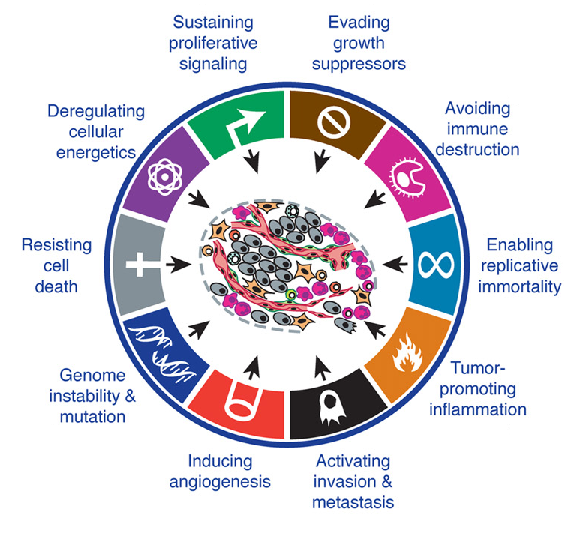
\includegraphics[width=0.55\textwidth]{Figures/Intro/hallmarks.pdf}
    \caption[The hallmarks of cancer]{\textbf{The hallmarks of cancer}. From Hanahan \textit{et al.} \cite{Hanahan2011}}
    \label{fig:intro_hallmarks}
\end{figure}
The first part of the introduction describes how genomic changes can influence cancer development and how the technological advances in the genomics area have enabled to shed lights on the mechanisms involved. 

\subsection{The central dogma of molecular biology}
%good videaos: https://www.youtube.com/watch?v=J3HVVi2k2No   https://www.khanacademy.org/test-prep/mcat/biomolecules/amino-acids-and-proteins1/v/central-dogma-of-molecular-biology-2
%\textit{"DNA makes RNA makes protein"}, Marshall Niremberg, Nobel price in Physiology and Medicine in 1968. \\

%Cancer complexity: from Genome to Proteome
At the beginning of the 19th century, Avery and colleagues isolated and identified the \gls{DNA} as the molecule constituting our chromosomes, defined previously as carriers of our hereditary material by Thomas Morgan \cite{Avery1944,Morgan}. In 1953, Watson and Crick proposed a new structure for the \gls*{DNA} molecule, the double helix structure \cite{Watson1953} (See Figure \ref{fig:intro_fig1}A). Five years later, Francis Crick formulates how the information contained in the sequence of nucleic acids is processed to produce the proteins needed by our cells in what is called the central dogma of molecular biology (Figure \ref{fig:intro_fig1}B-C). 
\begin{figure}[H]
    \centering
    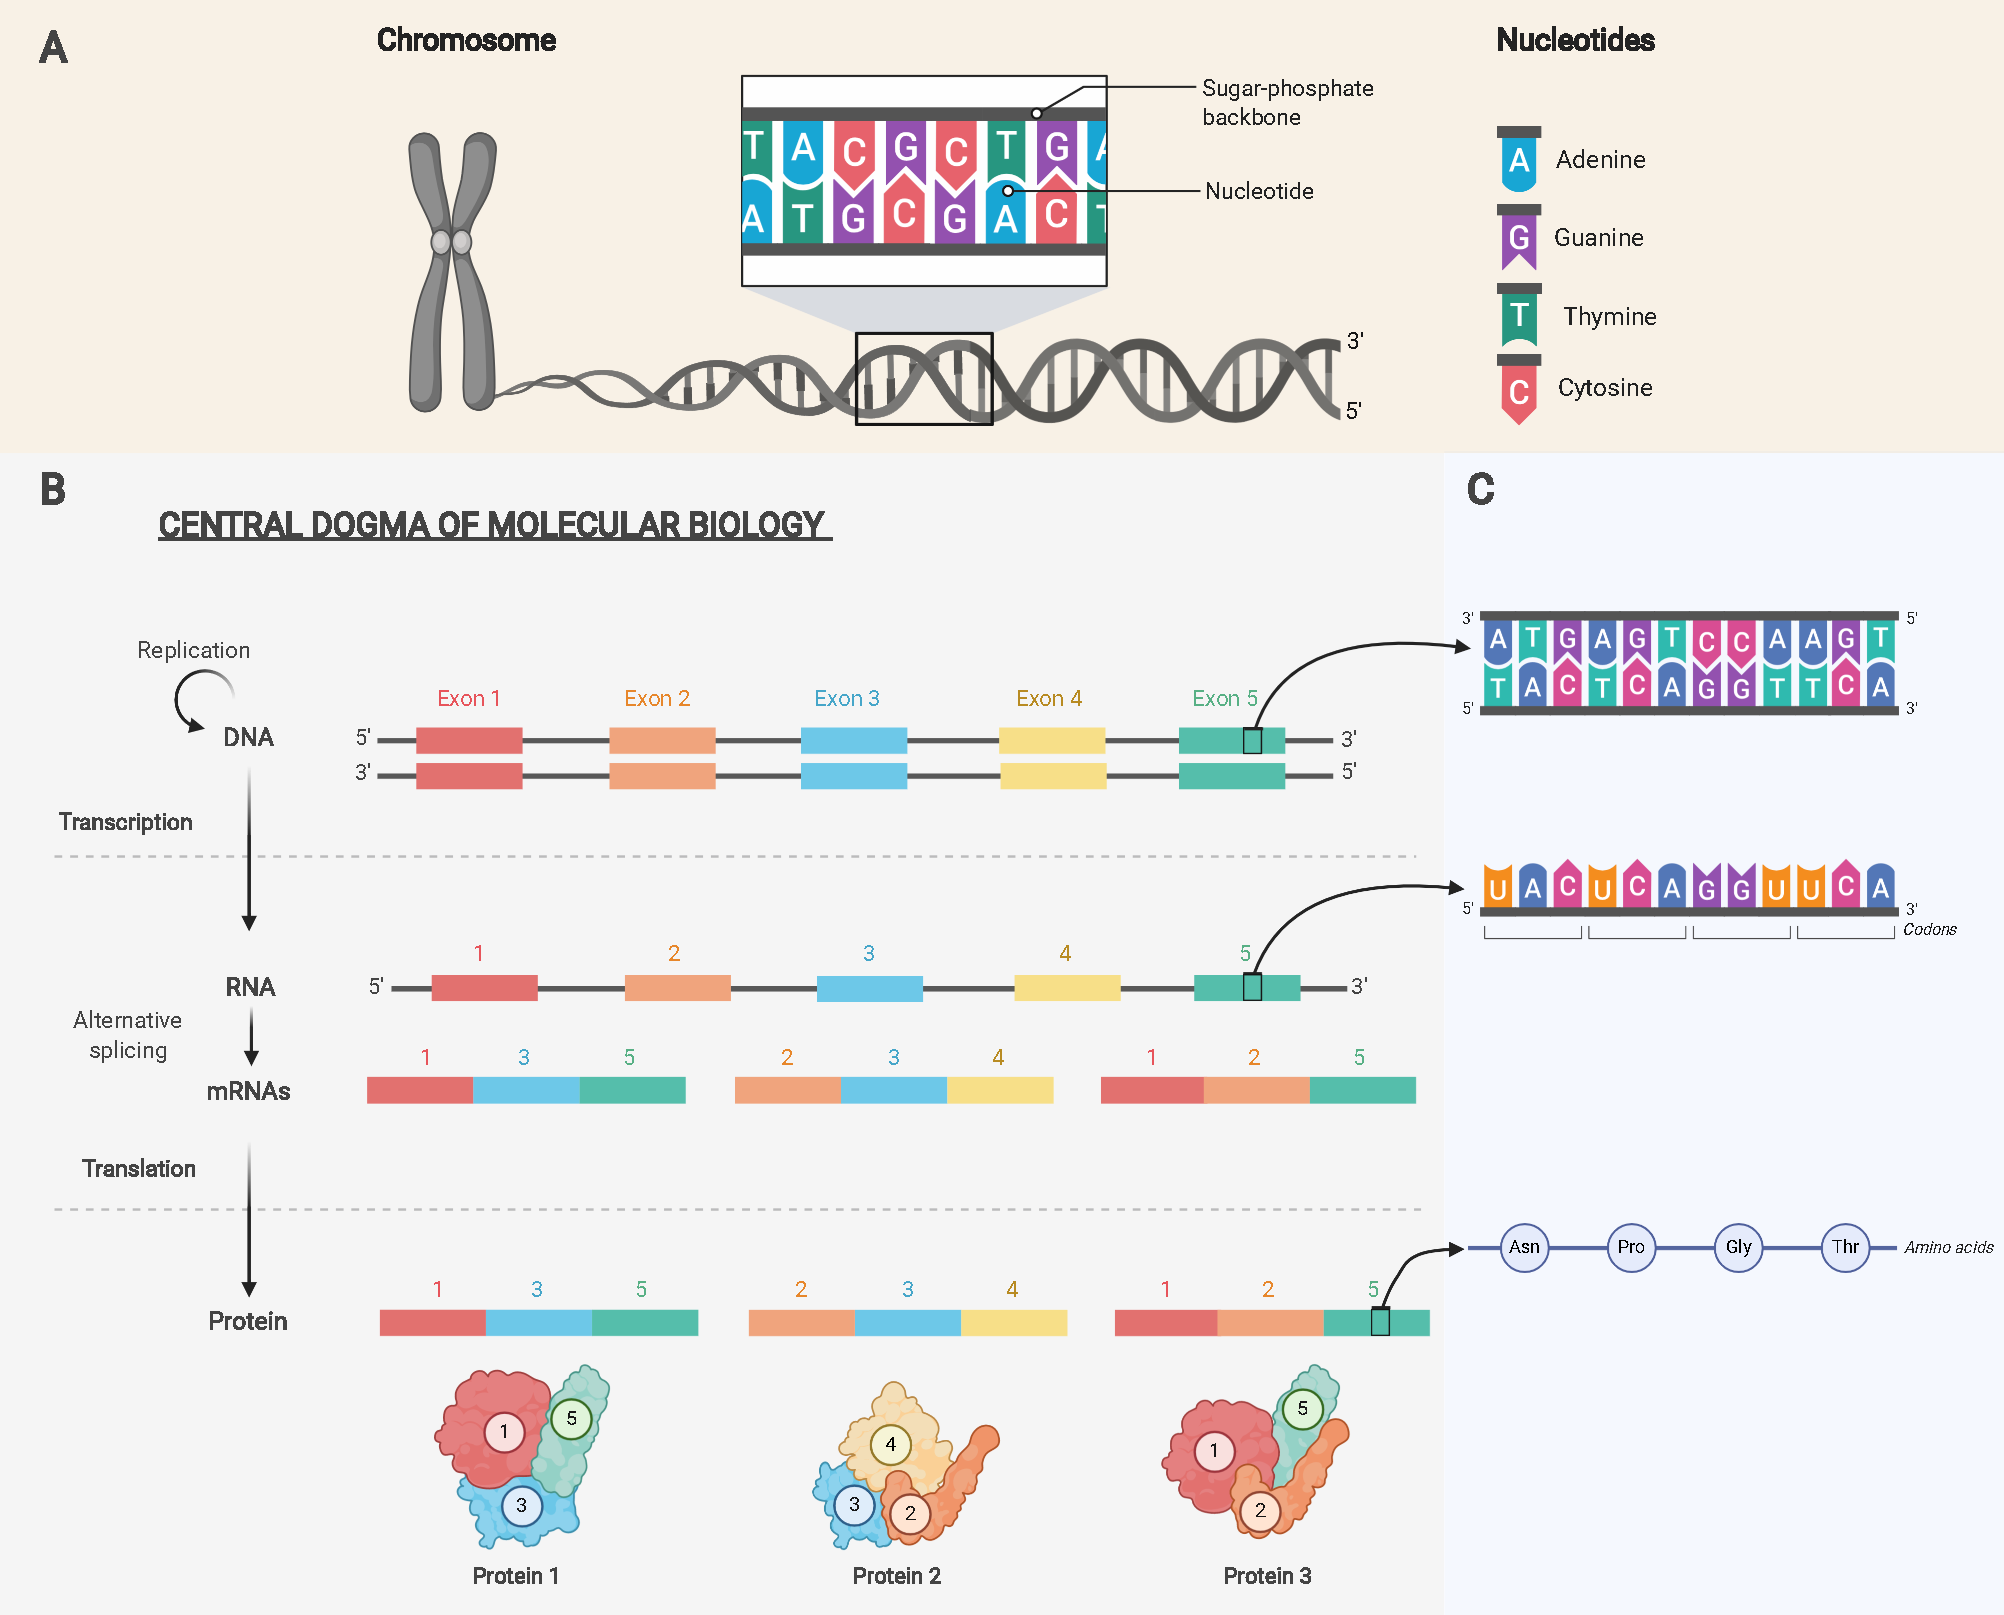
\includegraphics[width=0.95\textwidth]{Figures/Intro/Fig_1.pdf}
    \caption[The DNA molecule and the central dogma of molecular biology]{\textbf{The \gls*{DNA} molecule and the central dogma of molecular biology}. A) The structure of \gls*{DNA}: the double helix molecule is composed of two complementary strands of nucleotides. B) Representation of the steps described by the central dogma of molecular biology. C) Illustration of the molecules resulting from the central dogma transfers at a higher resolution. Created with \href{https://biorender.com/}{BioRender.com}}
    \label{fig:intro_fig1}
\end{figure}
Three main transfers are described by the central dogma: replication, transcription and translation (See Figure \ref{fig:intro_fig1}B). During replication, the \gls*{DNA} molecule is duplicated to provide the needed information to progeny cells. Through the two other steps, the information contained in \gls*{DNA} is used to generate proteins. Firstly, the process of transcription consists in reading the \gls*{DNA} sequence to synthesize a single-stranded molecule of the same length, the \gls{RNA}. During translation, the transcribed molecule is then read using a reading frame of three nucleotides that form what is called a codon encoding for one amino acid, the unit of a protein (See Figure \ref{fig:intro_fig1}C). Note that the genetic code is redundant; multiple codons can encode an amino acid. The conversion of the information encoded in our genes to functional gene products like proteins is referred to as gene expression.

%more complexity
Since the statement of the central dogma, other mechanisms have been identified as determinant for the expression of a protein. Firstly, the \gls*{RNA} molecule resulting from the transcription process, containing regions coding for the final amino acids sequence (exons) and non-coding regions (introns), is actually a \gls{pre-mRNAs}. The step transforming precursor \gls*{RNA} to mature \gls{mRNAs} is called alternative splicing and consists in truncating intronic regions and joining different exons together (See Figure \ref{fig:intro_fig1}B). Hence, one pre-mRNA can lead to multiple \gls{mRNAs} that are then transported outside of the nucleus to be translated into different proteins. While around 20,000 genes are described, much more proteins are generated as a result of alternative splicing.

% regulatory elements
Although all of our cells share the same genetic information and follow the same dogma, it is known that cells in distinct tissues differentiate and do not express the same proteins, at the same time. Such differences can be explained by the fact that several regulatory processes control gene expression levels.
Firstly, genes transcription is dependent on transcription factors that represent around 7\% of the genes \cite{Weinberg2014}. They specifically bind to control regions of genes,  provide or prevent access to the \gls*{DNA} and can control multiple genes \cite{Weinberg2014}. The fact that genes, for example the transcription factors, can influence multiple genes and thus multiple possibly unrelated phenotypes is referred to as pleiotropy.
After transcription, \gls{mRNAs} can also be regulated through other \gls*{RNA} molecules, like the \gls{miRNAs}, that can degrade \gls{mRNAs}. %Those micro-RNAs might explain why the mRNA expression levels do not always correlate with protein expression levels. 
% epigenetic events
Besides, differences in gene expression can be controlled via non-genetic mechanisms like epigenetic processes, including histone modifications and \gls*{DNA} methylation. Histones are proteins around which the \gls*{DNA} is wrapped and hence control \gls*{DNA} accessibility (Figure \ref{fig:intro_fig2}). For example, histone phosphorylation leads to the condensation of the chromatin and inhibits gene expression \cite{Weinberg2014}.
\gls*{DNA} methylation consists in the addition of a methyl group to cytosine nucleotides located in \gls{CpG} dinucleotides sites (cytosine followed by a guanine nucleotide). Such positions are not homogeneously distributed across the genome and are more frequently observed in what is called \gls{CpG} islands, themselves mainly observed in regulatory regions of genes, the promoters. It has been observed that the methylation of \gls{CpG} sites in promoters can repress gene expression while methylation of positions in the gene body positively correlates with gene expression \cite{Ma2013a}. 
\begin{figure}[H]
    \centering
    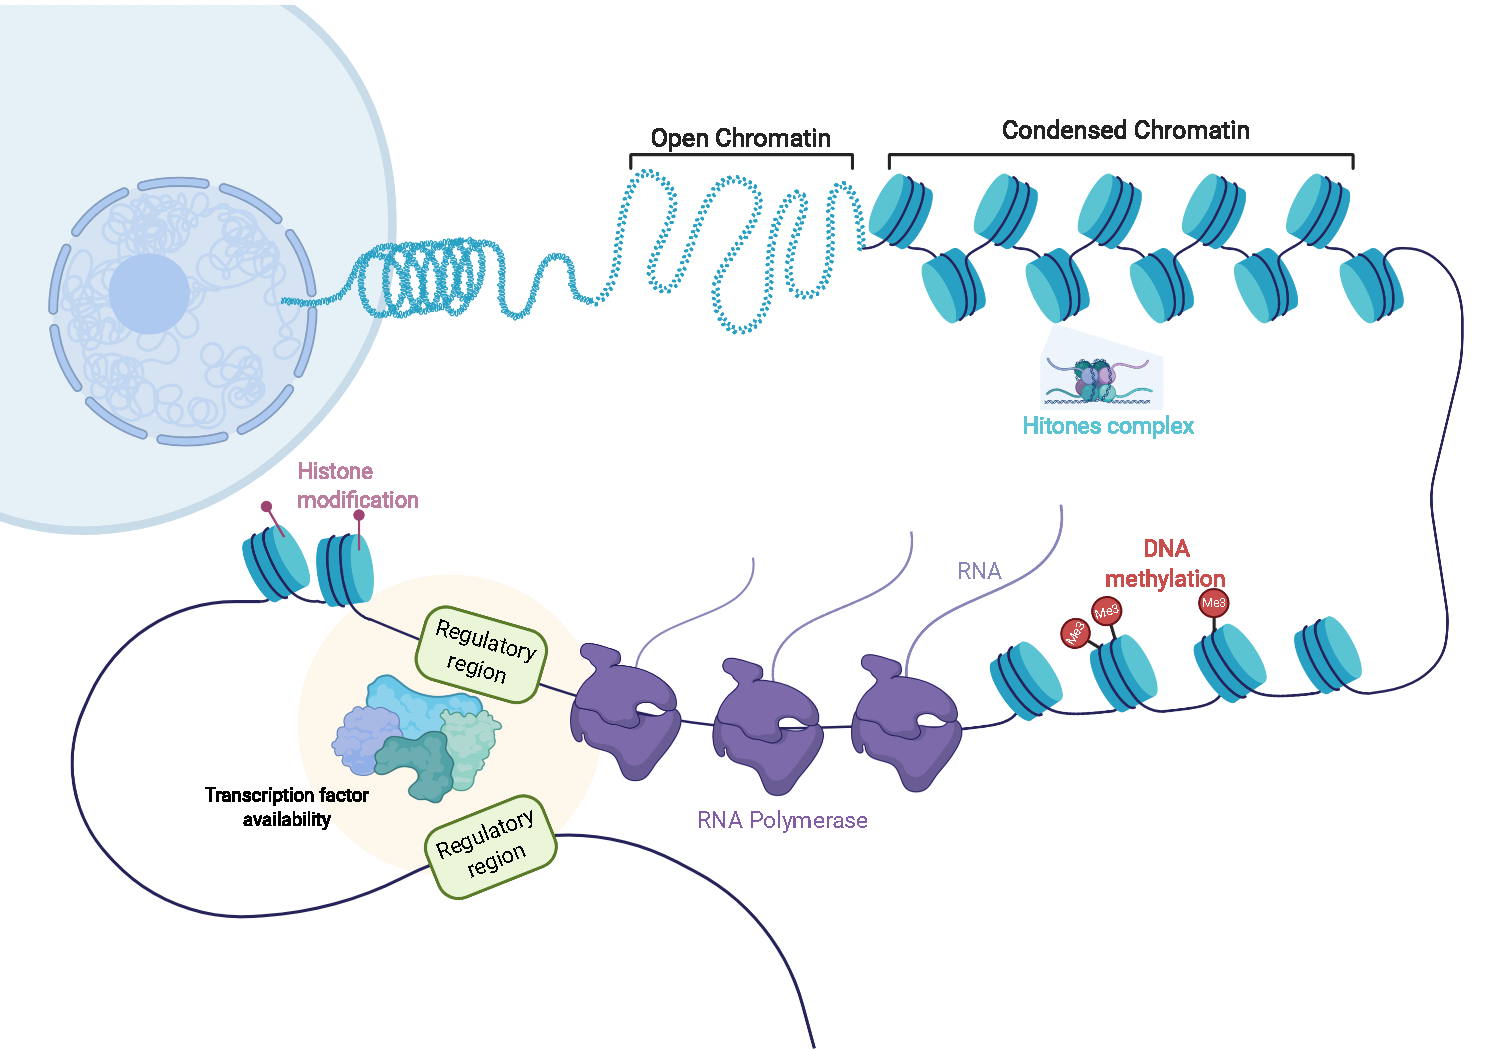
\includegraphics[width=0.8\textwidth]{Figures/Intro/transcription_regulation.pdf}
    \caption[Regulation of transcription]{\textbf{Regulation of transcription}. The figure represents different configurations of \gls*{DNA} packaging. The \gls*{DNA} molecule is wrapped around histones proteins that themselves are gathered in complexes called nucleosomes. This packaging forms the chromatin structure. This structure can be more or less compact (open versus condensed chromatin), which is influencing gene expression. When the chromatin is open, transcription factors can access the \gls*{DNA} molecule, and \gls*{RNA} polymerases can initiate the transcription. Note that the structure of the chromatin can be influenced by histones modifications and \gls*{DNA} methylation events. Created with \href{https://biorender.com/}{BioRender.com}}
    \label{fig:intro_fig2}
\end{figure}
Finally, post-translational events like enzymatic modifications of proteins or protein cleavage can occur and increase the number of proteins that can be generated in human cells, hence adding an additional layer of complexity.
% Impact on gene expression. For multiple tasks in the cells, translation, repairing DNA, replication, DNA must be open (euchromatin).
%house keeping genes vs tissue specific genes

%These elements highlight the complexity of the molecular mechanisms. There are even mechanisms that goes against the central dogma, for example the reverse transcription: we can go back to the DNA level; other example, non coding RNA that skip the step of translation.

As such, the numerous steps of transferring the \gls*{DNA} sequence information to proteins reflect the complexity behind protein expression. Any of these steps can be disrupted and result in altered molecules and proteins, leading to cancer development.  

\subsection{Cancer: a genomic disease}

%The previous section suggests that maintaining DNA integrity is critical to allow our cells to function properly. However, 
Our \gls*{DNA} continuously undergoes diverse alterations %altered what is called mutations 
and their accumulation over time can cause cancer. Researchers started to investigate the role of genomes in cancer at the end of the 19th century. In 1890, David von Hansemann, by observing cancer cell division under a microscope, identified for the first time abnormal chromosomes. This observation, among others, led Theodor Boveri 20 years later to suggest that cancer was a consequence of alterations in our inherited \gls*{DNA} \cite{Stratton2009}. His hypothesis was supported in the mid 20th century by the identification of a recurrent alteration resulting in a peculiar chromosome 22 (the Philadelphia chromosome), in \gls{CML}.
While those alterations have been observed at the chromosomal level, genomes can be impacted by a multitude of alterations detectable at a lower resolution, the modification of one nucleotide in the \gls*{DNA} sequence being the lowest resolution. 

At any position of the genome, the nucleotides might vary from an individual to another as well as between cells of an individual; those variations are called \gls{SNVs}. Also, larger events like nucleotides \gls{indels} of up to 1,000 bases and structural variations (chromosomal rearrangements or large \gls{indels}) can alter the \gls*{DNA} sequence. All of these genomic changes are called mutations.
\begin{figure}[H]
    \centering
    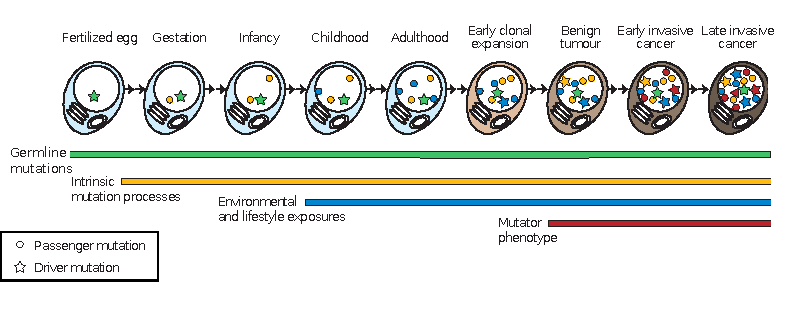
\includegraphics[width=1\textwidth]{Figures/Intro/Fig_mutation_over_life.pdf}
    \caption[The timing of somatic mutations acquisition]{\textbf{The timing of somatic mutations acquisition}. Mutations can be inherited at birth (germline mutations, in green) or acquired during life course (somatic mutations, in yellow, blue and red). They can have little to no impact (passenger mutations represented by circles) or confer an advantage to the cell (driver mutations represented by stars). Adapted from Stratton \textit{et al. } \cite{Stratton2009}}
    \label{fig:intro_fig3}
\end{figure}
%germline vs somatic alterations
Mutations can occur at different moments in life (See Figure \ref{fig:intro_fig3}). Some mutations are inherited at birth since they are present in the germ line cells (sperm and egg) transmitted by parents to the offspring. They are called germline mutations and are found in all the cells of an individual, normal cells as well as tumor cells. 
Such mutations are observed at different frequencies in different populations and are called \gls{SNP}s. %Note though that the notion of SNPs is usually extended to any germline variation. 
Another category of mutations can also be found in all cells of the body even if they were not transmitted by our parents, if they occur early in life during the development, at gestation. They are called \textit{de novo} mutations. Finally, the rest of the mutations found in humans are acquired later in life as a result of errors in the \gls*{DNA} maintenance or exogenous damages (See next section). Those mutations occur in cells outside the germ line and are called the somatic mutations. 
%In a human genome, each mutation type is not expected at the same frequency, a germline mutation is expected every 1,000 bases when somatic mutations every 1,000,000 bases approximately depending on the cancer type \cite{Alexandrov2013}. 

%impact of mutations
Also, whether they are germline or somatic, mutations can have different impacts. Most mutations have, due to the redundancy of the genetic code, little to no impact on the genes encoded around them, they are the passenger mutations \cite{Vogelstein2013}. Others though alter the gene product and confer a selective advantage to the cell, \textit{e.g.} a faster proliferation or a better survival in comparison to neighbour cells \cite{Stratton2009}. Those mutations are called driver mutations as they are thought to contribute to “driving the carcinogenic process” and are preserved by positive selection. In 2018, the Cancer Gene Census described more than 700 driver genes (genes carrying driver mutations). Among them, 90\% were associated with somatic mutations and 20\% contained germline mutations \cite{Sondka2018,CancerGeneCensus}. Generally, two types of driver genes exist, oncogenes and \gls{TSG}. 
Oncogenes are genes whose functions are to promote cell growth, proliferation or inhibit apoptosis and usually result from a gain of function. A mutation in an oncogene can thus lead to a deregulation of one of these processes, hence resulting in uncontrolled proliferation and cancer. The first mutation identified as causing cancer was discovered in 1982 by Reddy \textit{et al.} and was activating an oncogene named \textit{HRAS} \cite{Reddy1982}. Besides mutations, other processes like over-expression of genes via amplification or chromosomal translocations can activate this category of genes. 
%Some mutations can alter the gene product because they truncate the protein, some can impact the levels of expression (mention structural variants and copy number changes).  
In contrast to oncogenes, \gls{TSG}s are refraining cellular growth and proliferation and are often referred to as the "gatekeepers" genes. Mutations in \gls{TSG}s tend to result in a loss of function; the latter genes are inactivated, and their negative regulation of cell proliferation is cancelled, which leads to abnormal growth. 
In 1971, Knudson proposed the two hits hypothesis which stipulates that both alleles (versions of a gene inherited by our mother and father, identical alleles leading to the homozygous state while two different alleles to the heterozygous state) of a \gls{TSG} must be inactivated or lost for the gene to lose its normal functions \cite{Knudson1971}. This hypothesis seemed to explain familial cancer cases \cite{Martinez-Jimenez2020}. Indeed when the first hit is an inherited germline mutation, the cancer susceptibility of a person increases since only one alteration is needed to alter the \gls{TSG} functions. The second alteration can result from different events: a mutation in the second allele, the loss or translocation of chromosome pieces or the loss of an entire chromosome. The two latter events causing what is called \gls{LOH} \cite{Eggert2011}.
%the 3 hits hypothesis: Waszak et al. Nature 2020.

In the case of the two hits hypothesis, two mutations in the same gene are required for cancer initiation. However, it has been described that cancer is rather a multi-step process, meaning that multiple mutations and more than one gene are usually involved. %This multi-step facet of cancer is visible via the progressive histopathological states. 
A certain number of alterations in key pathways are necessary, and it can take several years for cancer to develop \cite{Weinberg2014}. However, the multi-step process can be accelerated. Firstly, as mentioned previously, the inheritance of germline mutations speeds up the cancer development as one driver mutation might be present from birth, increasing the probability that the remaining necessary events, which generally follow a stochastic process, will also occur. %since it can lead to the occurrence of a first driver mutation which, due to the low frequency of mutation events, is a rate-limiting event
\cite{Weinberg2014}. Also, even if multiple \gls*{DNA} repair mechanisms fix most of the alterations that a genome endures, the \gls*{DNA} repair pathways themselves can be disrupted, leading to an acceleration of the accumulation of alterations. Such an event increases the mutation rate of an individual and generates what is called a "mutator phenotype" \cite{Stratton2009,Loeb1991}. Finally, driver genes can also be altered by epigenetic changes that are more frequent, which increases the chance of disrupting key biological pathways for cancer development. 


\subsection{Cancer: an environmental disease}
Mutations can arise from endogenous processes, for example, errors happening during \gls*{DNA} replication. In that regard, the appearance of mutations across the genome seems random, and the advent of a driver mutation leading to cancer development seem associated with bad luck. This idea has been developed by Tomasetti \textit{et al.} \citep{Tomasetti2015} in a controversial paper, published in 2015, suggesting that the majority of cancer mutations were due to "bad luck". In 2017, the same authors confirmed that mutations due to random errors represent a large proportion of mutations in multiple cancers while specifying that if luck and randomness do play a role in cancer development, other factors like exogenous processes also impact our \gls*{DNA} and contribute to cancer development. \citep{Tomasetti2017}

Cancer incidence varies depending on the countries considered. Lung cancer incidence, for example, is much higher in Asia, Europe and North America than in Africa \cite{globocan_lung}. Those differences can be explained by the fact that cancer has a heritable component that differs in different parts of the world and by the fact that environmental exposures are different across countries. %and are in part responsible for cancer development. 
It has been shown, though, in studies exploring cancer rates in migrants populations, that the differences observed among populations could not be explained only by the genetic component \cite{Peto2001}.  
In the second half of the 20th century, epidemiological studies have indicated that several environmental exposures were associated with cancer incidence, showing that many cancers could be prevented. One of the most striking findings was that of Doll \textit{et al.} showing that smokers had a twenty-fold higher risk of developing lung cancer than non-smokers \cite{Doll1950}. At the same period, chemical agents have been identified as being able to induce cancer, \textit{i.e.} being carcinogenic \cite{Loeb2008}. Some of these agents were also defined as mutagenic agents, \textit{i.e.} agents inducing \gls*{DNA} damages. 

Some carcinogens can impact cancer evolution without causing \gls*{DNA} alterations; they are non-mutagenic agents and are considered as tumor promoters. One example of tumor promoter is alcohol which is a cytotoxic substance. %In contrast with tobacco smoke containing multiple mutagenic carcinogens, ethanol has a low mutagenic effect while being cytotoxic. 
Its consumption leads indeed to the death of epithelial cells in the mouth and throat, which triggers the division of the stem cells to regenerate the epithelium. If tobacco consumption precedes this event, tobacco-induced mutations might be present in the dividing cells, and clonal expansion of these mutations may lead to cancer \cite{Weinberg2014}. In that case, smoking acts as a tumor initiator and alcohol as a promoter by stimulating cell proliferation. Such interaction between alcohol and smoking is observed in head and neck cancers. Note, however, that alcohol can also have a mutagenic effect due to metabolites generated during ethanol oxidation like acetaldehyde \cite{Seitz2010}. Other examples of tumor promoters are steroid hormones acting as mitogenic agents or chronic inflammation (\textit{e.g.} due to viruses). 

% the mutator phenotype
%In the previous section, cancer was described as a multi-step disease that can take several years to develop. However, this time can be largely reduced by external factors like environmental exposures. Once cell starts acquiring mutations, the mutation rate can vary and increase, when DNA repair pathways are impacted for example, this create a "mutator phenotype" (see \cite{Stratton2009} and \cite{Loeb1991} to say that the mutator phetotype might be required to go through the multistage of the disease). An exposure can contribute to get the mutator phenotype  \cite{Yoshida2020}

%Mutational signatures
We have seen that mutations in our genome can result from endogenous processes like replication errors or \gls*{DNA} repair defects and from exposition to carcinogens. Observing these mutations across the whole genome have revealed patterns. Indeed, each of these processes can generate what is called mutational signatures, \textit{i.e.} specific combinations of mutations \cite{Alexandrov2013}. %Identifying mutational signatures in tumors can help to understand the etiology of the studied tumor. 
The first studies of mutational signatures focused on single base nucleotide substitutions (six possible substitutions: C$>$A, C$>$T, C$>$G,  T$>$A, T$>$C, T$>$G) and their tri-nucleotide contexts (the 5' and 3' nucleotides flanking the substitution) leading to 96 possible classes of mutations. The classification of all mutations found in cancer genomes in those 96 groups and the use of mathematical methods (See section \ref{Intro-method}) to decompose the mutational processes enable the identification of a limited but diverse set of signatures. In the case of lung cancers, comparing the DNA of smokers with that of non-smokers revealed an increase of mutations in smokers mainly due to an elevation of C to A (C$>$A) mutations, probably caused by the tendency of tobacco carcinogens to induce this particular change \cite{Nik-Zainal2015}. In melanoma samples, an increase of C$>$T substitutions has been identified as a result of \gls{UV} light exposition \cite{Alexandrov2014}. 
In 2015, COSMIC provided a curated set of 30 mutational signatures based on previously published studies on different cancer types \cite{Cosmic_2015}. Recently the methods to disentangle mutational signatures in human genomes have been extended. In 2020, Alexandrov \textit{et al.} have considered higher context to classify single base substitutions by considering two flanking bases around the positions of the mutations and analyzed as well other types of mutations like double base substitutions and \gls{indels}. This work led to an expansion of the repertoire of mutational signatures with more than 60 signatures in total \cite{Alexandrov2020}. %Some signatures have been decomposed, like the Apobec signature. Note though that the origin of some signatures are still unknown. 
%Organ specific signatures exist (see signal.mutationalsignatures.com). 

Although some signatures are resulting from endogenous processes, like defects in \gls*{DNA} repair or unknown processes, multiple signatures have been associated with preventable exposures. %, meaning that many cancers could be prevented. 
Considering the important impact of environmental exposures, Wild \textit{et al.} suggested in 2005 the concept of the \textit{exposome} which corresponds to all the exposures encountered by an individual during his lifetime (\textit{e.g.} life-style, exposures to chemicals). He expressed the need to improve the measurement of such exposures at the same scale of the genomic events measurements \cite{Wild2005}. %in order to better understand cancer etiology and improve cancer prevention \cite{Wild2005}. 
Indeed on the genome side, remarkable technological advances were made in the past decades allowing researchers to explore the human genome at high resolution. The evolution of these technologies is described in the next section.

% exposures can also affect methylome: https://clinicalepigeneticsjournal.biomedcentral.com/articles/10.1186/s13148-019-0713-2
%Environment can also influence the methylation profile. (see slide from zenko on bees and the fact that twins have different profile while environmental exposures are different)

\let\clearpage\relax



%----------------------------------------------------------------------------------------
%	SECTION 1
%----------------------------------------------------------------------------------------
\section{The era of genomics}
\label{Intro-ngs} 
\subsection{From arrays to next generation sequencing} %From genotyping to sequencing
%https://www.researchgate.net/publication/279833953_Analysis_of_Somatic_Alterations_in_Cancer_Genome_From_SNP_Arrays_to_Next_Generation_Sequencing
%Paper "the cancer genome" \url{https://www.nature.com/articles/nature07943} Discovery of cancer genes 
%https://www.intechopen.com/books/next-generation-sequencing-advances-applications-and-challenges/next-generation-sequencing-an-overview-of-the-history-tools-and-omic-applications#B3

The identification of the genomics variations leading to cancer has been enabled by multiple technical and technological advances that occurred after the discovery of the \gls*{DNA} structure. Since that discovery, researchers have attempted to decipher the hidden information contained in the double helix molecule. 
One fundamental advancement in genomics has been the development of the first generation sequencing by Frederic Sanger in the 1970s. After automatization, this technique led indeed to the sequencing of the first human genome in the context of the \gls{HGP} that started
%2020 marked the 20th anniversary of the Human genome project (HGP) that enabled the sequencing of the first human genome.  
in the 1980s, took 13 years and cost around 3 billion dollars to lead, in 2003, to the sequencing of the 3 billion nucleotides that our \gls*{DNA} constitutes. At that time, the largest genome sequenced was the 20,000 times smaller genome of the Epstein-Barr virus \cite{Roberts2001}. While many researchers thought it was impossible, the project completed and delivered the first version of the human genome reference which, after being revised and improved, is now used on a day-to-day basis in genomics.
%The time needed to analyze and understand it is much longer. Diagnoses of many diseases have changed a lot based on the sequencing of the DNAs patient. Understanding of predisposition. Understanding of the mechanisms, causes of cancer.
%In 2007, four years only after the completion of the HGP project, James Watson was the first one to have his genome sequenced for less than 1 million dollar \cite{Check2007}. %Watson genome sequenced \cite{Gyles2008}
However, the first generation sequencing technology was too long and costly to be applied in larger research projects aiming in that period to catalogue the genetic variations involved in human diseases.

\subsubsection*{The array technology}

At the same period, the microarrays technologies were far less expensive. This technique consists in disposing, on an array, \gls*{DNA} sequences, called probes, designed to bind (by hybridization) to target sequences in a sample. The target sequences are labelled to measure the hybridization and quantify the target molecules. %One of the main use of microarrays was to measure the expression levels of specific genes in cells under different conditions. 
\begin{figure}[H]
    \centering
    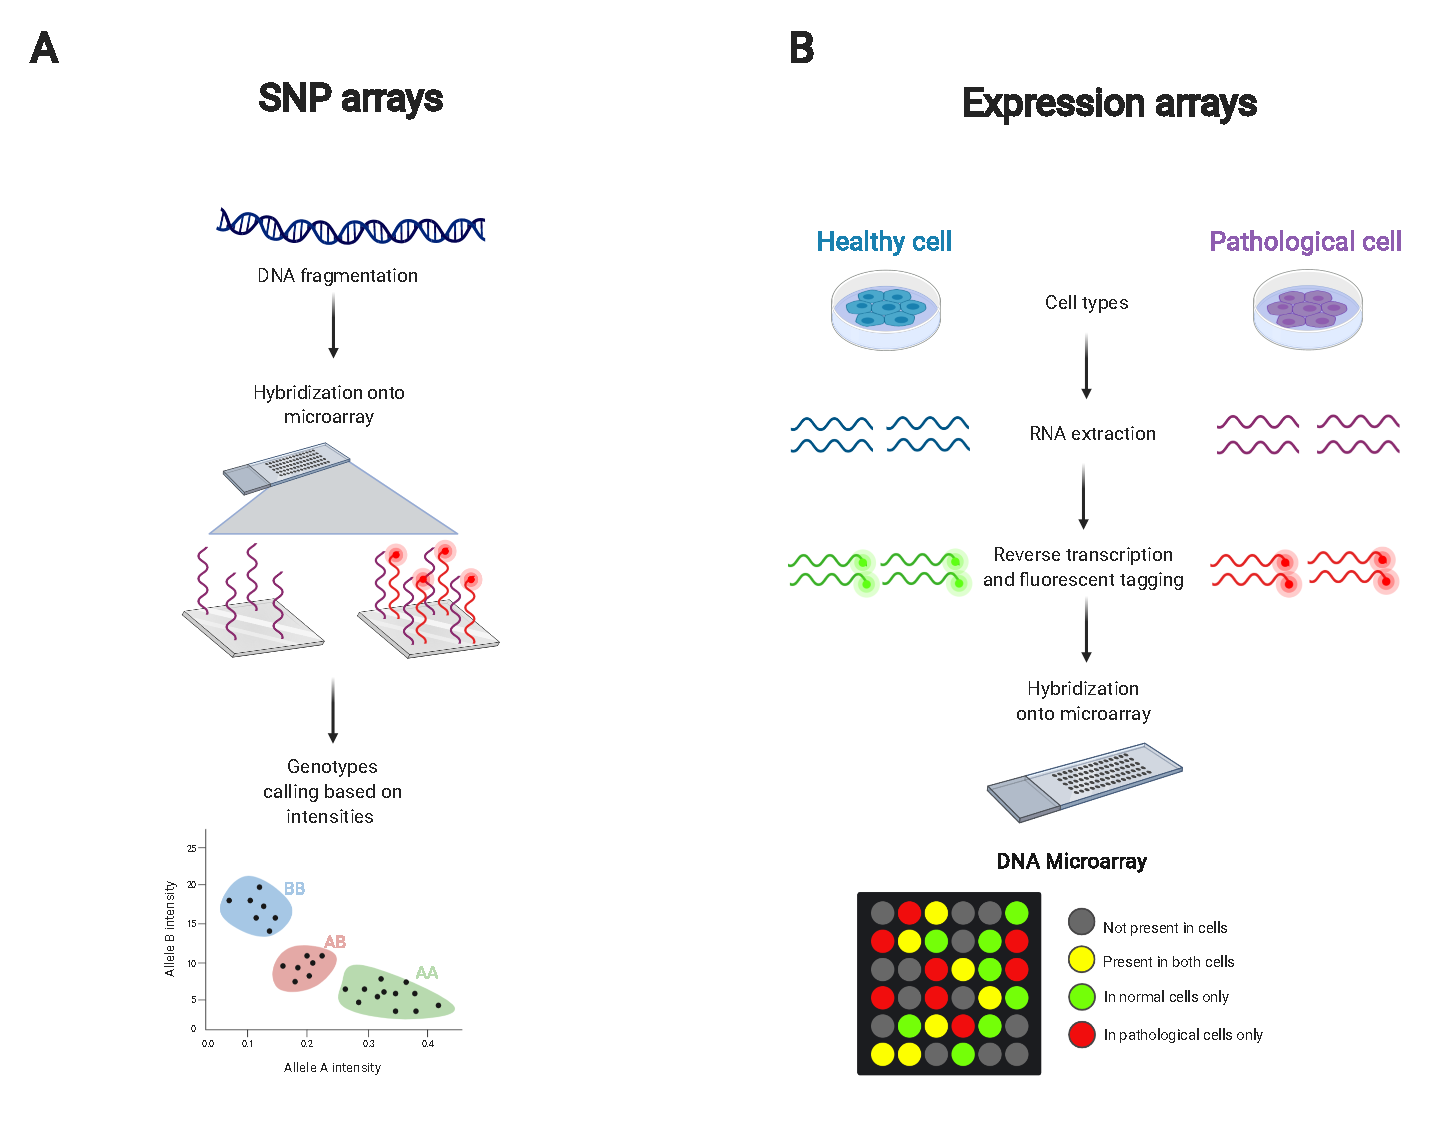
\includegraphics[width=0.9\textwidth]{Figures/Intro/arrays.pdf}
    \caption[Microarrays]{\textbf{Microarrays}. A) \gls*{SNP} arrays: fragmented \gls*{DNA} sequences bind to designed probes on the microarray, which generates an intensity signal that varies depending on the allele carried by the \gls*{DNA} sequences. B) Expression arrays: tagged complementary \gls*{DNA}, reverse-transcribed from \gls{mRNAs} molecules, bind to gene-specific probes, which generates a fluorescence signal used to compare expression levels in different cell conditions. Created with \href{https://biorender.com/}{BioRender.com}}
    \label{fig:intro_arrays}
\end{figure}
In order to study genomic variations across the genome, specific microarrays were developed, the genotyping or \gls*{SNP}s arrays. Those arrays contain unique probe sequences, targeting specific positions of the genome, which hybridize to single-stranded \gls*{DNA} that has been fragmented. This generates intensities signals varying depending on the allele carried by the \gls*{DNA} sequence binding to each probe. This intensity, indicating the presence or absence of each allele, is then converted into genotypes \cite{Laframboise2009} (See Figure \ref{fig:intro_arrays}A). %The first SNP array developed for commercial purposes was the Affymetrix array that has evolved over time to interrogate from 10,000 to 500,000 SNPs.
The \gls*{SNP} arrays developed for commercial purposes have evolved, interrogating from 10,000 to millions of sites simultaneously in a given individual \cite{Xing2016}. Key produces of these technologies were developed by Affymetrix and Illumina inc. Those arrays have been used so far for different purposes. They allowed the identification of copy number changes or, for arrays with high marker density regions, the detection of \gls{LOH} events by identifying regions without heterozygous positions \cite{Beroukhim2006,Dutt2007}. They have also been used to identify germline variants that associate with a certain disease through \gls{GWAS} \cite{XueyingMao2007}. As illustrated in Figure \ref{fig:intro_gwas}, \gls{GWAS} interrogate millions of positions across the genome by testing their association with
a specific trait, like smoking traits, individually and reveal positions significantly associated with that trait.  
\begin{figure}[H]
    \centering
    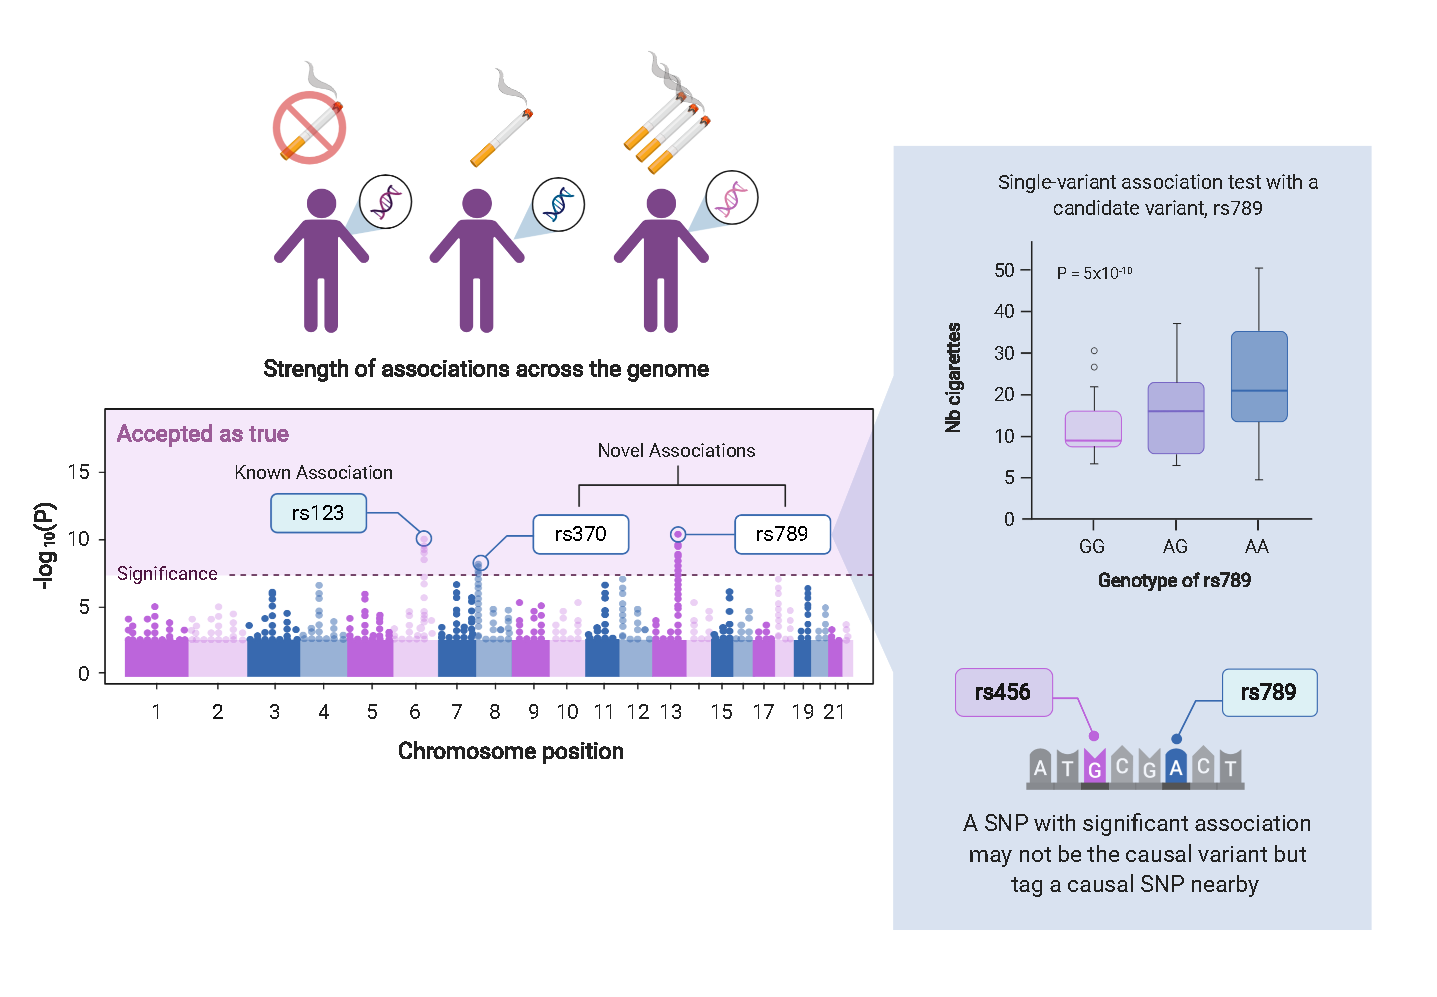
\includegraphics[width=1\textwidth]{Figures/Intro/GWAS.pdf}
    \caption[Genome-wide association studies]{\textbf{Genome-wide association studies}. The figure illustrates a \gls{GWAS} identifying \gls*{SNP}s associated with the number of cigarettes smoked per day. For each position, the association between the variant genotypes and the number of cigarettes per day is tested (rs789 example). The associations \textit{p}-values are represented in a Manhattan plot (left panel). \gls*{SNP}s reaching the genome-wide significance threshold of $5.10^{-8}$ are considered as true associations. Those \gls*{SNP}s do however not always correspond to the causal variant but often tag a nearby \gls*{SNP} in linkage disequilibrium. Created with \href{https://biorender.com/}{BioRender.com}}
    \label{fig:intro_gwas}
\end{figure}
%Today, SNP arrays have the capacity to genotype millions of positions, \textit{e.g.} around five millions markers for the Omni5 array \cite{Xing2016}. 
%Other use of SNP arrays, determining the samples ancestry, which is important in the identification of disease related SNPs. Indeed ....
Although \gls*{SNP}s arrays are limited to the positions assayed, much more positions can be studied based on the arrays. Indeed, \gls*{SNP}s are transmitted to the offspring linked to other close \gls*{SNP}s in blocks called haplotypes. This relationship between \gls*{SNP}s is called \gls{LD}. Knowing the \gls*{SNP}s composition of a haplotype enables to predict the genotype of \gls*{SNP}s that were not assayed by the array by using the information of the assayed positions in the haplotype. Hence, genotyping hundred thousands of \gls*{SNP}s allows actually to impute the genotype of millions of other variants thanks to \gls{LD}. The definition of the haplotypes required though to study such genomic structure in different samples to build a map as reference. Those were the goals of the \gls{HapMap} started in 2002 \cite{Belmont2003,Hapmap_britannica}.

% read this to have ideas on the limitations: https://medium.com/the-gencove-blog/it-is-time-to-replace-genotyping-arrays-with-sequencing-73535efa66ed
%First catalogue of human variation was the HapMap (haplotype map) project. \\

Micro-arrays platforms have also been used to study the other molecular layers like the transcriptome and the methylome. For the analysis of the expression profile, micro-arrays have enabled to measure and compare the expression levels of specific genes in cells under different conditions, \textit{e.g.} diseased versus healthy cells or treated versus non-treated cells. Figure \ref{fig:intro_arrays}B describes the main steps of an expression array experiment. The extracted \gls{mRNAs} molecules from both types of cells, after being reverse-transcribed to \gls{cDNA} and labelled with fluorescent dye, hybridize to the genes specific probes fixed on the array. The array is then scanned using fluorescent imaging \cite{Tarca2006}. The fluorescence amount detected at each probe is proportional to the amount of \gls{mRNAs} in cells. While these measures do not provide absolute quantification of gene expression levels, they enable to compare the expression levels in the different conditions.
%methylation techniques
%Arrays and sequencing methods have allowed to explore the genetic information stored in our DNA. Similar technologies 
Arrays have also been used to study the epigenome by allowing the detection and the analysis of methylation events. The most commonly used methylation arrays are the Illumina arrays \cite{Illumina_Methylation_infinium}. As for the \gls*{SNP}s arrays, probes are designed to target specific loci of the human genome, in this case, \gls{CpG} positions. The number of positions interrogated by such arrays can vary from 25,000 to 850,000 positions depending on the array (\textit{e.g.} Illumina 25K, 450K and 850K arrays). Probes are designed and fixed to the array to bind to both methylated and unmethylated loci (Figure \ref{fig:intro_methylation}). This binding is enabled by a chemical process called bisulfite conversion, which converts unmethylated cytosines to uracil and leave methylated cytosine unchanged. At the hybridization step, a single-based extension is performed with labelled nucleotides, allowing to distinguish for each locus a methylated vs non-methylated signal (Figure \ref{fig:intro_methylation}). The ratio between the two signals at a locus provides a value, called $\beta$ value, which indicates the level of methylation. This value ranges between 0 and 1, 0 corresponding to a non-methylated and 1 a methylated position. 
\begin{figure}[H]
    \centering
    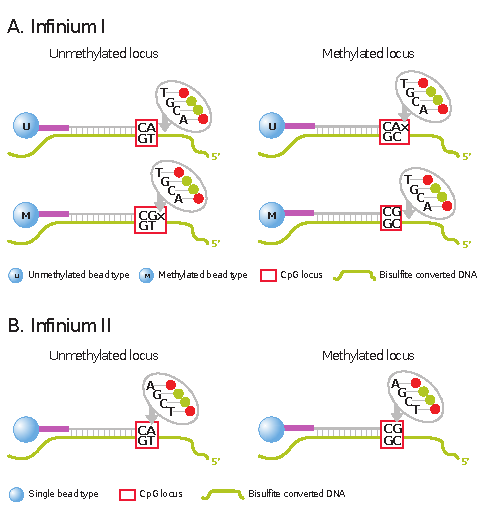
\includegraphics[width=0.8\textwidth]{Figures/Intro/Illumina_methylation2.pdf}
    \caption[The Illumina Infinium methylation assay]{\textbf{The Illumina Infinium methylation assay} (From \cite{Illumina_Methylation_infinium}). This figure represents the probes used for methylation profiling by Illumina. A) Infinium type I probes. Two site-specific probes are found on the array: probes allowing methylated sites with the preserved cytosine to bind (methylated bead M) and probes designed for the unmethylated site with the thymine nucleotide resulting from bisulfite conversion and whole-genome amplification (methylated bead U). B) Infinium type II probes. Only one probe per locus is required to bind to both methylated and unmethylated sites. In that case, single-base extension with labelled nucleotides is used.}
    \label{fig:intro_methylation}
\end{figure}

% read this: https://www.gesundheitsindustrie-bw.de/en/article/news/dna-from-watson-and-crick-to-modern-molecular-biology
\subsubsection*{Next-generation sequencing}
While the \gls*{SNP} arrays enabled to access the genotype information of millions of positions, there was still a need to re-sequence human genomes more efficiently and access the complete \gls*{DNA} sequence to better identify genetic variations. Around 2005, the second generation of sequencing methods called \gls{NGS} has been developed. 
\begin{figure}[H]
    \centering
    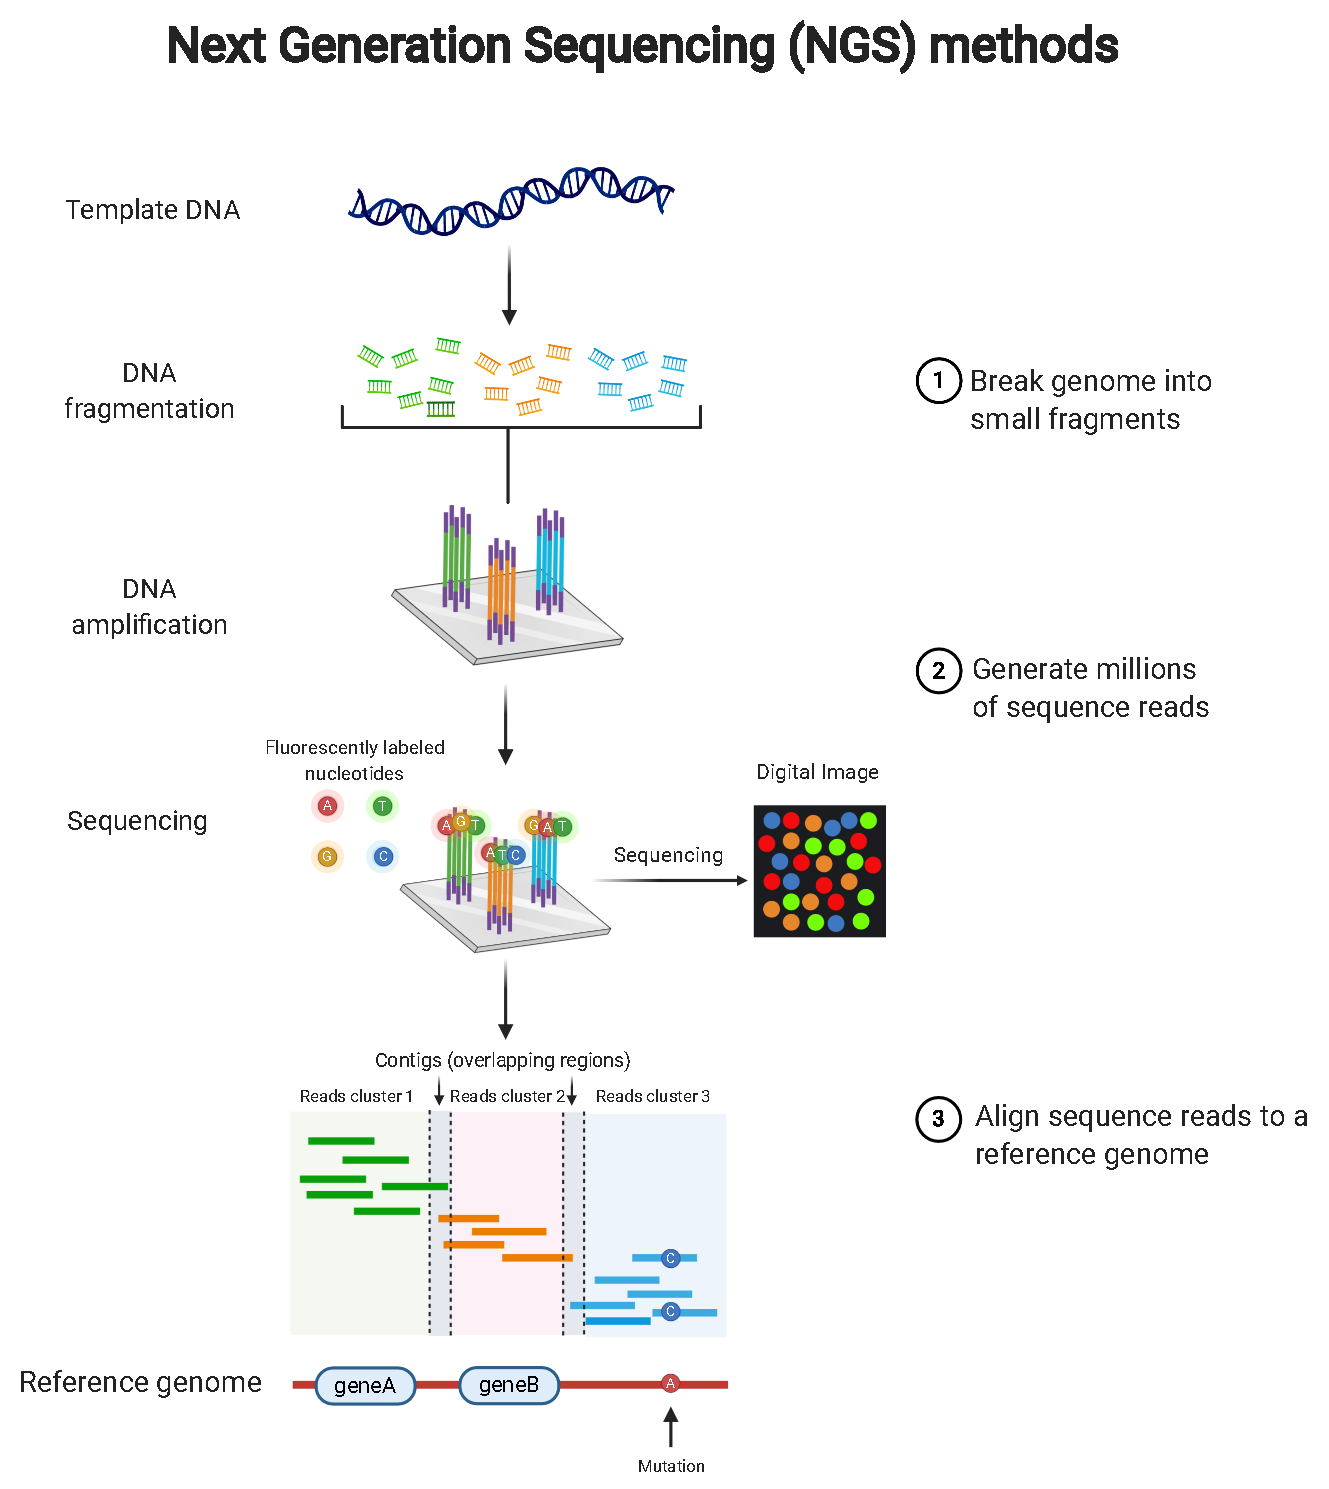
\includegraphics[width=0.8\textwidth]{Figures/Intro/ngs.pdf}
    \caption[Next Generation Sequencing methods]{\textbf{Next Generation Sequencing methods}. The figure describes the \gls{NGS} steps consisting in: i) fragmenting the nucleic acid molecule, ii) amplifying the fragments (using \gls{PCR}), iii) sequencing the resulting copies using single-base extension that adds one after the other labelled nucleotides whose signals are detected using digital imaging. The sequencing reads are then aligned to a reference genome to assemble the reads in a single sequence or to detect mutations across the genome. In the case of \gls*{RNA} sequencing, the reads align to exonic regions of the genes and they are counted to quantify gene expression levels. Created with \href{https://biorender.com/}{BioRender.com}}
    \label{fig:intro_ngs}
\end{figure}
The main change in these new methods in comparison to the first one was the parallelization of the sequencing, which allowed to produce millions of sequences, called reads, at the same time and hence to decrease drastically the time of sequencing as well as its cost \cite{Wetterstrand} (Figure \ref{fig:intro_ngs}). 
\gls{NGS} methods enabled the rapid re-sequencing of different parts and lengths of the genome. The entire genome sequence (except some highly problematic regions) can be accessed with \gls{WGS}. The restricted sequencing of coding regions (exonic regions) can be performed with \gls{WES}. Finally, it is possible to sequence specific regions of the genome, usually genes, using targeted sequencing. 
Based on these techniques, bioinformatics methods have been developed to detect germline as well as somatic variants. They consist in mapping (or aligning) the sequenced reads to a reference genome, and positions that vary from the reference are identified as variations (Figure \ref{fig:intro_ngs}). A mismatch between a sequenced genome and the reference genome is expected around every 1,000 bases. To distinguish somatic from germline mutations, both tumor and normal cells \gls*{DNA} from the same individual have to be sequenced. The tumor \gls*{DNA} is compared to the normal \gls*{DNA} and variations found in the tumor cells only are classified as somatic mutations. Somatic mutations are expected every 1,000,000 bases approximately depending on the cancer type \cite{Alexandrov2013}. 

While the \gls*{DNA} sequencing techniques have been used to detect \gls*{DNA} mutations, they do not explore the expression or methylation layers.
In 2008, the sequencing of the \gls*{RNA} molecule (\gls{RNA-Seq}) had been performed to study expression profiles. In this technique, the \gls{mRNAs} molecules are fragmented and converted to complementary \gls*{DNA} before sequencing, and the resulting reads are aligned to the reference genome \cite{Wang2009}. After the alignment step, the reads can be assigned to genes and the abundance of reads mapped on a gene, quantified using the number of mapped reads, reflects the expression level of the gene (Figure \ref{fig:intro_ngs}). A high read count value indicating that a gene is active and transcribed in that sample. The comparison of the read counts distributions in samples from different conditions, \textit{e.g.} samples with and without disease or diseased samples under different treatment, can be used to identify genes involved in or causing a specific condition. \gls{RNA-Seq} can also be used to identify different transcripts of a gene as well as gene rearrangements like translocations. 

Note that other recent techniques, while not described in the thesis, also exist to access different omics layers. A new sequencing technique has been developed for the analysis of the methylome, the bisulfite sequencing, which in contrast with the methylation arrays, can interrogate millions of \gls{CpG}s positions across the whole genome as well as positions in targeted regions. Also, the study of chromatin accessibility and \gls*{DNA}-binding proteins is possible thanks to \gls{ATAC-seq} and Chromatin immunoprecipitation experiments followed by sequencing (\gls{ChiP-Seq}) respectively \cite{Furey2012,Yan2020}. Finally, while the sequencing methods presented so far process \gls*{DNA} coming from a bulk of cells, single-cell sequencing methods have been developed to perform molecular characterization at the cell level. These methods allow the identification of distinct populations of cells in a tumor and hence the study of tumor heterogeneity and tumor microenvironment \cite{Hwang2018,Finotello2019}.
%The ability to detect the somatic variations in the entire genome of tumor cells have expanded the discovery of driver genes. 
%the 1000 genome dataset that sequenced ... from 26 different populations across the world. This property is used in imputation methods which attempt to estimate the missing genotypes on an array \cite{Marchini2010}. 

The decreasing costs of genotyping and sequencing methods have enabled the establishment of genomics studies involving large cohorts \cite{Wetterstrand}. Sequencing a human genome today costs less than 1,000 dollars using \gls{NGS} methods while it would still cost millions if the Sanger method was chosen. Multiple research groups have coordinated their efforts to create large consortia for that purpose and in many cases have shared the resulting data to the scientific community. The next section provides an overview of some of these initiatives.


\subsection{Large public databases}
%the 1000 genome dataset that sequenced ... from 26 different populations across the world. This property is used in imputation methods which attempt to estimate the missing genotypes on an array \cite{Marchini2010}. 

\subsubsection*{The Cancer Genome Atlas}
\gls{TCGA} is a public database providing access to 10,000 patients whose tumors have undergone multi-omics characterization. The project was launched in 2005 by the \gls{NIH} and aimed at characterizing the genomic alterations underlying several cancer types. For that purpose, multiple omics data were generated \cite{Tomczak2015}. The tumor and normal samples from most of the \gls{TCGA} participants have been sequenced using \gls{WES}. Based on these data, multiple variant callers have been used to catalogue the germline and somatic mutations present in each sample. Genotyping has been performed to analyze copy number variations. The transcriptome of most samples has also been sequenced, using \gls*{RNA} and \gls{miRNAs} sequencing. The methylation profiles of the tumors were explored with the use of 25K or 450K methylation arrays. Finally, protein expression profiling has been performed based on \gls{RPPA}. In addition to the molecular data, clinical and environmental exposures data were collected when possible. The \gls{TCGA} projects also delivered the histopathological images associated to each tumor. Based on these diverse omics and clinical datasets, "marker papers" describing the molecular landscape of each tumor type have been published. While the tissues explored at the beginning of the initiative were limited to lung, brain and ovaries, the \gls{TCGA} data encompasses today molecular data from 33 different cancer types. Those cancer-specific studies led to the identification of genomics alterations causing each cancer type, hence the discovery of new driver genes and potential cancer biomarkers, \textit{i.e.} molecules found in the body as an indicator of a disease or specific condition. Also, cancer subtypes were characterized on the molecular level and subtype-specific alterations were identified, which resulted in new clinical managements of tumors \cite{Weinstein2013}. In parallel to the cancer-specific studies, the \gls{TCGA} research network launched, in 2012, the Pan-Cancer Atlas initiative aiming at exploring the commonalities between cancer types, distinguishing tissue-specific determinants of cancer as well as increasing the statistical power for the identification of genomic alterations \cite{Weinstein2013}. This initiative was completed in 2018 and the data have been released and associated to 27 papers, published in Cell, focusing on three main topics: i) cell-of-origin patterns and cancers subgrouping, ii) oncogenic processes, and iii) signaling pathways involved in cancer \cite{PanCanatlas_site}. 

\subsubsection*{The International Cancer Genome Consortium (ICGC) initiatives}
The \gls{TCGA} studies focused their efforts on the characterization of the cancer exomes. However, exomes represent only 1\% of the human genome and much more can be discovered by exploring the remaining 99\% of the genome. In 2007, the \gls{ICGC} project was launched to study more than 20,000 whole genomes from 50 cancer types having an impact in multiple regions of the world (the 25k initiative).  The international consortium aimed at generating a catalogue of the somatic mutations in those cancer types, sharing the resulting datasets and complementing them with transcriptomic and epigenomic datasets \cite{Hudson2010,Cieslik2020}.
%\subsubsection*{Pan-Cancer Analysis of Whole Genomes (PCAWG)}
Based on the samples included in the \gls{TCGA} and the \gls{ICGC} projects, the \gls{PCAWG} project, an \gls{ICGC} initiative also know as the Pan-Cancer project, has arisen \cite{Campbell2020}. The project relied on more than 2600 samples from 38 different tumor types and aimed at meta-analyzing whole-genome data across cancers along the same lines as the PanCancer Atlas project. The first results from these data have been released in 2020 in a series of publications in Nature \cite{Cieslik2020}. While the \gls{TCGA} initiative enabled the study of the coding regions of the samples, the \gls{PCAWG} project, thanks to the use of whole genome sequences, was designed to explore broader mutational patterns in the coding and non-coding regions, from small to large events like structural variations. For example, chromoplexy and chromothripsis events, which are complex chromosomal rearrangements resulting from catastrophic genomic events, have been observed in more cancers than expected, 17.8\% and 22.3\% of the tumors, respectively \cite{Cieslik2020}. Also, one major result from the \gls{PCAWG} project has been the expansion of the mutational signatures mentioned in section \ref{Intro-biology} \cite{Alexandrov2020}, as well as the discovery of 16 structural variants signatures \cite{Li2020}. 
%The PCAWG genomes were complemented by RNA sequencing data for more than 1000 samples \cite{Cieslik2020}.
%Example of the study of the impact of somatic SVs on genome topology and gene regulation Northcott et al. Nature 2014. 
%Ghavi-Helm et al. Nat Genet 2019: SVs 

% germline
\subsubsection*{UKbiobank}
The previously described projects mainly targeted the somatic landscape of genomes. Other large projects have enabled the research community to explore the germline component of human disease. The largest public dataset, focusing on germline genetics, has been generated by the UKbiobank project, which started in 2010 in the UK. This project gathered data from a population-based cohort of around 500,000 participants between 40 and 69 \cite{Bahcall2018} and had as main objective to improve our understand of the interaction between genetics and multiple human diseases. For that purpose, all participants were genotyped. Besides, multiple other biological samples, like urine, blood and saliva as well as physical measures, \textit{e.g.} brain \gls{MRI}, heart and eye measurements, were collected. It is a prospective cohort; participants are followed up and are linked to electronic health records \cite{Bycroft2018}. The genotyping data of the full cohort were released in 2017. Based on this dataset and the large panel of phenotypes, a multitude of \gls{GWAS} studies related to human diseases have been performed and their resulting summary statistics were made available. In 2019, around 100 \gls{GWAS} studies resulting from the UKbiobank data were available on the \gls{GWAS} catalogue, which provides curated \gls{GWAS} summary statistics results \cite{Buniello2019}. The follow-up of the patients has established that, in 2018, 79,000 of the participants were diagnosed with cancer \cite{Bycroft2018}, which means that cancer-related traits can also be studied using this dataset. After the release of the genotyped and imputed data, \gls{WES} and \gls{WGS} sequencing of the samples have been initiated. Part of the exome data, around 50,000 exomes, have already been released and about 200,000 exomes should be expected by the end of 2020. These data foreshadow future key findings in genomics, a better understanding of molecular and phenotypic interactions and probably an improvement of the translation of those findings in the clinic.% Similarly to the UKbiobank projects, multiple national genomics projects have started worldwide. In France, for example, in the context of the "France médecine génomique 2025" project, two sequencing plateforms were launched in 2017 and the sequencing of around 40,000 genomes is expected every year \cite{France_medecine_genomique}. 


\subsubsection*{Data sharing}
With the increasing number of genomics studies, public repositories, like the \gls{dbGAP}, the \gls{EGA} or \gls{GEO}, have been established to store petabytes of genomics data that can be accessed by the research community. In addition, large projects, like the \gls{TCGA} and \gls{ICGC}, have worked on solutions to improve data storage and accessibility.  %For example, all the \gls{TCGA} data have generated ... terabytes and the genomes sequenced through the \gls{PCAWG} project around 800 terabytes of data. 
One of the goals of those projects was to promote open-access data and the development of tools to foster the reuse of the data by the research community \cite{Weinstein2013,Hudson2010}. In 2010, the \gls{TCGA} provided the data in open access for the first time \cite{TCGA_milestones} and updated and extended the content of the open access data over the years. In 2016, the \gls{GDC} was launched by the \gls{NCI} to store all the \gls{TCGA} data \cite{Jensen2017}. For each omics, the data are categorized by levels: low-level data (raw and unnormalized data) that generally enable individuals re-identification are under controlled access, while higher-level data (processed data, clinical data) that do not permit re-identifiability are available without any requirement. In addition to providing the data storage, the \gls{GDC} also aimed at harmonizing and sharing the bioinformatics pipelines used to process the data \cite{Jensen2017,Gao2019}. The processed data resulting from the PanCancer Atlas papers are also available via the \gls{NIH} \gls{GDC} website \cite{PanCancerAtlas_data} and allow researchers to explore broader genomic features like immune variables \cite{Thorsson2018} or biological pathway measures \cite{Knijnenburg2018}.
Also, cloud computing solutions have been developed to facilitate the analyses of large public genomic datasets while avoiding the download and duplication of the data. The \gls{TCGA} and \gls{ICGC} data are available and can be analyzed on the cloud, for example via the \gls{CGC} \cite{Lau2017} or the \gls{ISB-CGC} \cite{Reynolds2017}. Also, the \gls{ICGC} consortium, to process the \gls{PCAWG} data, has developed a computational tool, Butler, which simplifies genomic analyses that have to be run on clouds environments (academic or commercial) \cite{Yakneen2020}.  \newline

In the past decades, the development of genomics technologies and the implementation of large consortia have enabled to characterize human cancers on the molecular level. The understanding of cancer causes and the biological mechanisms underlying tumor development has been improved. Also, due to the identification of correlations between molecular events and patient's prognosis and response to treatments, molecular studies have impacted the way that tumors are classified and managed in the clinic. 

\begin{comment}
Use of reproducible bioinformatics pipeline (e.g nextflow, give versions, github use, notebooks, docker), cloud computing
Example of data sharing \cite{Phillips2020}
Paper on genomic data sharing in europe: \cite{Saunders2019} 
use citations from \cite{Langmead2018}
\end{comment}



\section{The example of lung cancer}
\label{Intro-lung}
\subsection{Lung cancer subtypes and etiology}
\begin{figure}[H]
    \centering
    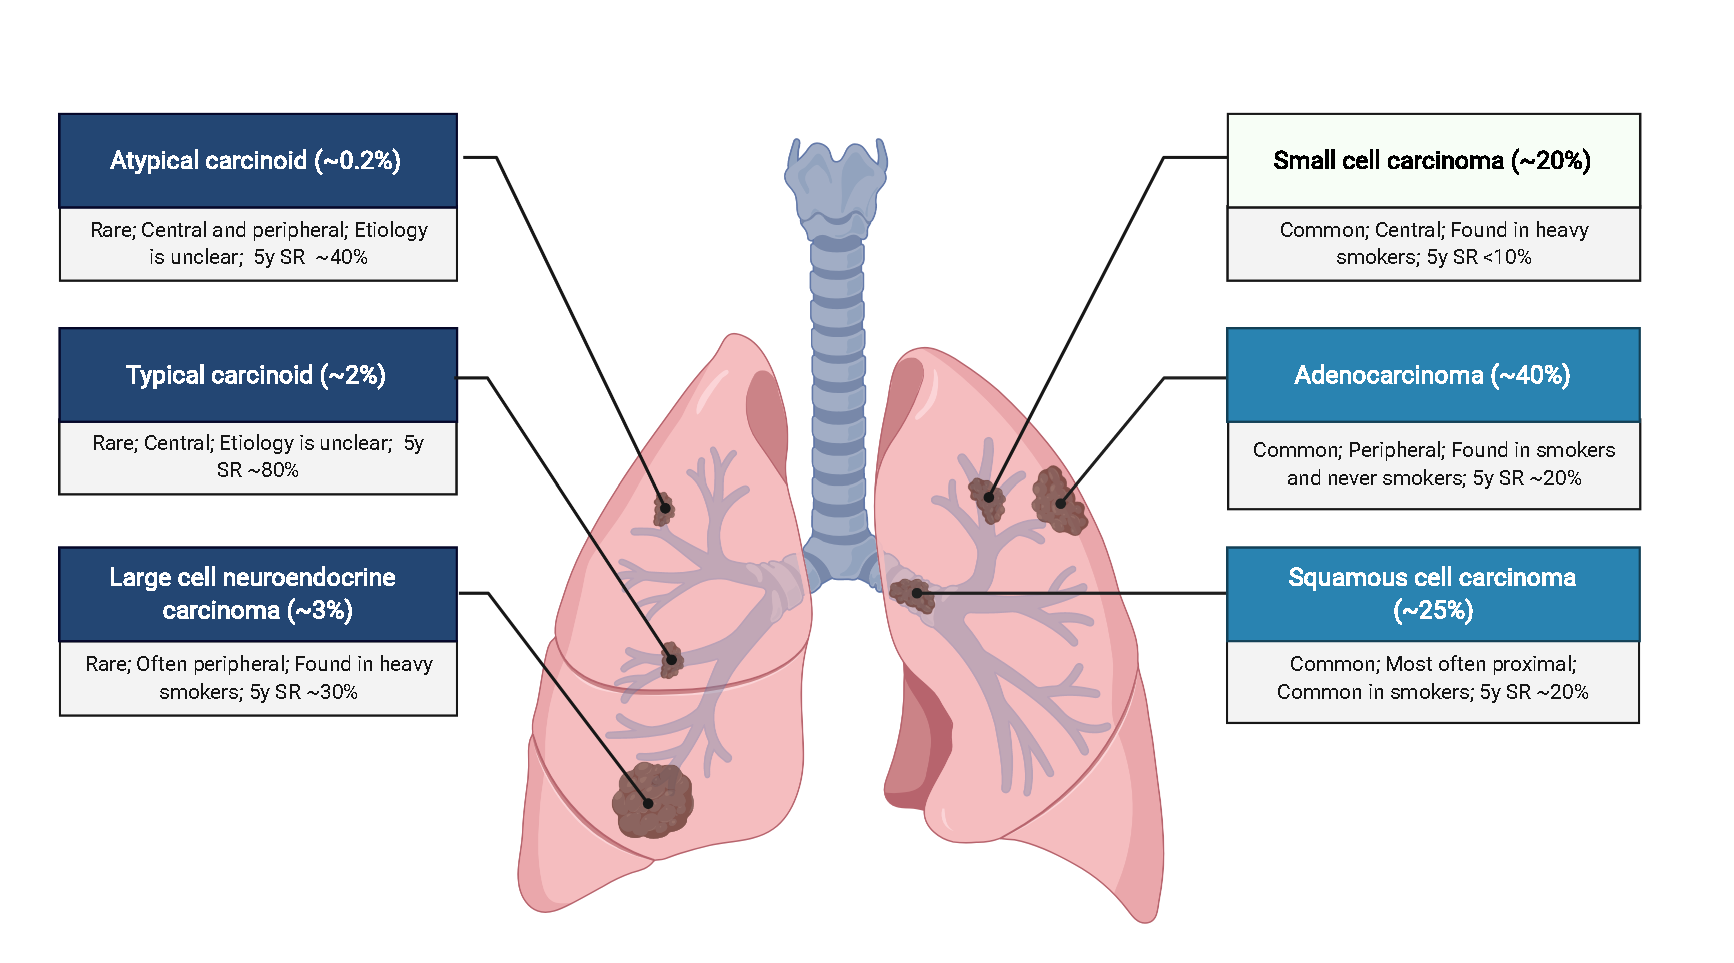
\includegraphics[width=1\textwidth]{Figures/Intro/Lung_cancer.pdf}
    \caption[Lung cancer subtypes]{\textbf{Lung cancer subtypes.} Each lung cancer type occurs at different frequencies as well as at distinct locations in the lung (from proximal to distal locations). Each box on the figure is associated to one cancer type and provides their characteristics (frequency, localisation, etiology and overall 5-year survival rate (5y SR)) \cite{Travis2010,Derks2018,Simbolo2019a,ASCO}. Figure created with \href{https://biorender.com/}{BioRender.com}}
    \label{fig:intro_lung}
\end{figure}
As mentioned at the beginning of the manuscript, lung cancer is one of the most common and deadliest cancer worldwide. Several subtypes of lung cancers have been identified (Figure \ref{fig:intro_lung}).
% Subtypes
The most common lung cancers are usually divided into two groups: the \gls{SCLC} and the \gls{NSCLC} samples, representing respectively around 20 and 75\% of the lung cancers \cite{Politi2015}. The second group is further separated into two main subgroups: the \gls{LUAD} and the \gls{LUSC}. Also, rarer forms of lung cancer exist. Multiple lung cancer subtypes, including such rarer cancers, were grouped in one category named the lung neuroendocrine tumors by the \gls{WHO} 2015 classification \cite{Travis2015}. This group comprises the pulmonary carcinoids, including the typical and atypical carcinoids, \gls{LCNEC} as well as the previously mentioned \gls{SCLC} tumors. 
Each lung cancer type can be distinguished by different etiologies, histopathological characteristics, molecular profiles and clinical outcomes (See Figure \ref{fig:intro_lung}).

%etiology
The strongest risk factor for lung cancer is smoking. Indeed, \gls{SCLC}s and \gls{LCNEC}s are frequently found in heavy smokers. Smoking is also a major risk factor for \gls{LUAD} and \gls{LUSC} cancers \cite{Campbell2016}. However, lung cancer can also develop in non-smokers. In particular, the \gls{LUAD} category corresponds to the lung cancer type most commonly found in never smokers. Although the etiology of the pulmonary carcinoids is not clear, the majority of these tumors are found in nonsmokers \cite{Derks2018}. %In addition, the smoking behaviour of patients from different subtypes can be different \cite{Pikor2013}...  
In addition, around only 15\% of smokers develop lung cancer suggesting than other factors mediate lung cancer risk. 

\subsection{Lung cancer susceptibility}
% Susceptibility
While exposures other than smoking like air pollution, radon, heavy metals or asbestos have been identified as lung cancer risk factors \cite{DeAlencar2020}, genetics is also contributing to the disease risk. In line with this hypothesis, it has been shown that having a family history of lung cancer confers a 2.5 fold lung cancer risk increase \cite{Amos1999}. Further evidence of lung cancer germline susceptibility has been revealed by \gls{GWAS} studies, with the identification of common variations associated with lung cancer. Genes involved in nicotine addiction (\textit{CHRNA} genes), telomere activities (\textit{TERT}) as well as genes related to the DNA repair and cell-cycle pathways (\textit{e.g.} \textit{Check2}, \textit{RAD52} or \textit{CDKN2A}) have been identified \cite{Bosse2018}. 
Also, some lung cancer associated variants were identified as related to the propensity to smoke \cite{Thorgeirsson2008,McKay2017} and genetic correlations between lung cancer and smoking traits, like smoking initiation, smoking cessation or smoking intensity have been described \cite{McKay2017}. Such observations provided evidence that susceptibility variants could influence lung cancer risk through environmental exposures.
Hence, \gls{GWAS} studies have enabled to gain insights on lung cancer etiology as well as on the biological pathways involved in the disease. However, the variants identified so far do not account for most of the heritability of lung cancer, estimated at 18\% and remaining today largely unexplained \cite{McKay2017}.  
%mention the ILCO consortium and TRICL
%inherited lung cancers \cite{DeAlencar2020}

\subsection{Lung cancer molecular profiling}
%mutational landscape
%Genetic studies like GWAS focus on germline genetics. 
In the past decades, molecular profiles of human tumors, including lung tumors, have also been explored thanks to the development of \gls{NGS} studies. Such studies have, for example, established that lung cancers are among the cancer types with the highest mutational burden (total number of mutations for a given part of \gls*{DNA}) \cite{Lawrence2013}.  
As mentioned in Section \ref{Intro-biology}, in smoking-related cancers, those mutations revealed a signature associated with tobacco consumption. Among the \gls{COSMIC} signatures identified by Alexandrov \textit{et al.} \cite{Alexandrov2013,Alexandrov2020}, the smoking signature corresponds to the Signature 4 (\gls{COSMIC} version 2) and SBS 4 (\gls{COSMIC} version 3). Those signatures are the results of \gls*{DNA} damages caused mainly by benzo[$\alpha$]pyrene, which is a mutagenic compound found in tobacco smoke and whose effects on \gls*{DNA} has been shown in experimental mutagenesis studies \cite{Nik-Zainal2015}. Even though smoking does heavily impact the lung tissue, it has been shown that quitting smoking can restore the damaged tissue \cite{Yoshida2020}.

In addition, molecular analyses of lung tumors have identified cancer driver genes in the different cancer types. Among those genes, the \textit{\gls{EGFR}} gene, which is part of the protein kinase family currently known to be mutated in around 15\% of the \gls{LUAD} samples \cite{Collisson2014}, has been related to therapeutic response in 2004 \cite{Politi2015}. Indeed LUAD samples, carrying activating mutations in the \textit{\gls{EGFR}} gene, are responsive to tyrosine kinase inhibitor therapy and have an improved survival in comparison to other cancer patients treated with chemotherapy. Such molecular studies largely influenced the way that lung tumors are classified since it is only since those discoveries that \gls{NSCLC} are further sub-classified. Guidelines were published in 2013 to include molecular testing, mainly based on \textit{\gls{EGFR}} and \textit{ALK} alterations testing, in the clinical practice for the \gls{NSCLC} patients. In 2018, those guidelines were updated and new alterations, like rearrangements in the tyrosine kinase \textit{ROS1}, are now recommended for molecular testing \cite{Lindeman2018}. In 2012 and 2014, the \gls{TCGA} marker papers on the two lung cancer cohorts (\gls{LUAD} and \gls{LUSC}) were published. The authors expanded the molecular profiling of these tumors and hence the list of drivers genes, improving the understanding of the biological mechanisms involved and providing new opportunities for patients management \cite{Network2012,Collisson2014}. Those studies also explored the transcriptomic, methylation and proteomic data from the lung tumors. Based on their expression profiles, the \gls{LUAD} tumors, were divided into subtypes that could help to refine those tumors classification \cite{Collisson2014}.

The identification of driver genes in lung cancer has also led to the proposal of molecular targets for early detection. The molecular profiling of \gls{SCLC}s is an example of such an application. \gls{SCLC}s are characterized by universal inactivation of both \textit{RB1} and \textit{TP53} genes \cite{Peifer2012a,George2015,Fernandez-Cuesta2019}. In 2016, Fernandez-Cuesta \textit{et al.} analyzed \gls{ctDNA}, which are fragments of tumor \gls*{DNA} released in the bloodstream that can be used as molecular biomarkers, in \gls{SCLC}s. They showed that \textit{TP53} mutations were detectable in the \gls{ctDNA} of the \gls{SCLC} cases \cite{Fernandez-cuesta2016}. 
\gls{ctDNA} applications are viable for multiple cancer types. In 2018, Cohen \textit{et al.} described a blood test called CancerSEEK, detecting proteins and mutations in cell-free \gls*{DNA} for the early detection of eight different cancer types, including lung cancer \cite{Cohen2018}. Such tests face though sensitivity issues due to the low abundance of mutated \gls*{DNA} in body fluids, hence adapted bioinformatics tools are needed. I contributed to the optimization of such tool, Needlestack, a highly sensitive multi-sample variant caller \cite{Delhomme2020}. 

Even though rare forms of lung cancers are less explored than the common lung cancers, recent molecular studies have started to characterize the lung neuroendocrine tumors as well \cite{Fernandez-Cuesta2014,George2018,Rekhtman2016,Simbolo2019}. Those studies have revealed that, on top of their histopathological differences, the lung neuroendocrine neoplasms were also distinct molecular entities \cite{Fernandez-Cuesta2019}. Low mutational burden has been observed in the atypical and typical pulmonary carcinoids in contrast to the highly mutated \gls{LCNEC}s and \gls{SCLC}s \cite{Derks2018}. Also, the transcriptomic profiling of those tumors has been investigated. These analyses identified molecular subgroups in different cancer types, revealing the molecular heterogeneity in those tumors \cite{George2018,Rudin2019}. The work described in chapters \ref{Chapter1} and \ref{Chapter2/4} of this thesis contributed to the molecular characterization of the lung neuroendocrine tumors.  \newline


The discoveries described in this section were enabled thanks to the large amount of data generated during the era of genomics (See Section \ref{Intro-ngs}). However, the analyses of these data have raised multiple challenges that required the use and development of specific computational methods. The next section intends to describe those aspects. 



%-----------------------------------
%	SECTION 1
%-----------------------------------
\section{Interpreting high dimensional data}
\label{Intro-method} 
The evolution of genotyping and sequencing technologies led to the generation of high dimensional datasets. In Section \ref{Intro-ngs}, we have seen for example that arrays can interrogate thousands to millions of positions across the genome and that sequencing techniques can provide the entire genome sequence or the expression levels of thousands of genes. While the amount of information unveiled by these methods is colossal, it can also bring about several challenges and adapted computational methods are required to analyze and interpret the data. The issues resulting from high dimensionality are associated to what is called the curse of dimensionality, firstly introduced by Bellman in 1961 and stipulating that the number of samples needed to interpret high dimensional data analyses appropriately increases exponentially with the number of dimensions \cite{Altman2018}.  
In omics datasets, even though large cohorts have been implemented (see section \ref{Intro-ngs}), the number of variables (also known as features), $p$, to analyze can be largely superior to the number of samples, $n$, included in the study. This introduces the $n<<p$ problem, which leads to multiple issues.
Firstly, usual statistical models like regression models need to be adapted since they require $p<n$. There is also a substantial amount of noise in the generated data that can mask the true signal in the data, \textit{i.e.} not all the measured features are of interest \cite{Domingos2012, Ronan2016}.
In addition, when the number of dimensions increases, the data points can occupy a more voluminous space and a larger proportion of this space will be empty, we say that the data are sparse (See Figure \ref{fig:intro_highdim}) \cite{Altman2018}. High data sparsity influences basic properties to which we are used to in two or three dimensions like distances. In high dimensions, distances between points increase and all points seem at the same distance from each other \cite{Ronan2016,Altman2018}. Also, the higher the dimensions, the lower the correlations between the features will be. %For those reasons, it is thus statistically more difficult to identify groups of points with similar characteristics, and larger sample sizes are required. 
For those reasons, it is thus statistically more difficult to identify groups of points with similar characteristics compared with random events, as such larger sample sizes are required to distinguish meaningful relationships. Another issue resulting from high dimensionality is multi-collinearity. Since the number of features is high, the information they carry can be correlated and become redundant; some variables might be defined as a linear combination of others which makes the data interpretation more difficult \cite{Altman2018}. 
Finally, the nature of omics datasets complicates the visualization of the data.
In this section, we will discuss in a first instance different strategies to explore such complex datasets and secondly focus on methods that attempt to diminish the problem of the curse of dimensionality: the dimensionality reduction methods.

%Mention pvalue correction and the new discussion about pvalues and confidence intervals on twitter.
%Problem also of quality of the data, measurement errors

\begin{figure}[H]
    \centering
    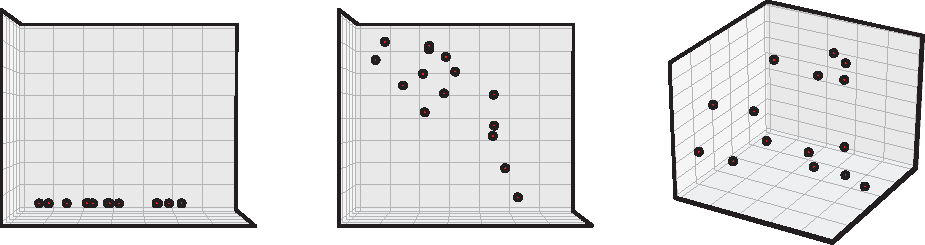
\includegraphics[width=0.8\textwidth]{Figures/Intro/high_dimentionality.pdf}
    \caption[Illustration of data sparsity]{\textbf{Illustration of data sparsity.} Figure from \cite{Ronan2016}. The figure represents how the data occupy the available space when going from a one-dimensional space to two and three-dimensional spaces (from left to right panels). }
    \label{fig:intro_highdim}
\end{figure}

\subsection{Supervised and unsupervised methods}

%Machine learning

Different approaches exist to analyze high dimensional data like omics data. In the case where specific biological hypotheses need to be tested, confirmatory data analyses based on inference models can be used. It can also happen that there are no predefined hypotheses and that the goal is to "let the data talk", in that case, \gls{EDA} will be more adapted \cite{Holmes}. A broad panel of statistical methods exists to assist both approaches. Among them, a large proportion can be grouped in the popular category of machine learning methods.  %In each case, different machine learning methods can be applied. 
The term \gls{ML} was used for the first time by Arthur Samuel around 1950 and defined a group of computer algorithms able to learn without being explicitly programmed to learn. Depending on the definition of learning, different classes of \gls{ML} methods have been established. In 1997, Tom Mitchell proposed a formal definition of algorithms learning saying that "A computer program is said to learn from experience E with respect to some class of tasks T and performance measure P if its performance at tasks in T, as measured by P, improves with experience E." \cite{Mitchell1997}. This definition matches a class of \gls{ML} methods, the supervised learning methods, used for classification and regression tasks. A common example is the identification of spam emails, where labelling emails in the spam or non-spam categories would be the task T, learning from a set of labelled emails would be the experience, and the proportion of correctly classified emails would be the performance measure P. However, \gls{ML} algorithms that simply learn from the input dataset without predefined ground truth (labelled data) also exist and are part of the unsupervised \gls{ML} methods. Those methods learn underlying structures in the data; hence algorithms like clustering or dimensionality reduction methods such as \gls{PCA}, which was developed even before \gls{ML}, are often included in the unsupervised learning category.
In the next paragraphs, both supervised and unsupervised learning are described (See Figure \ref{fig:intro_supervisedVSunsupervised}).  

\begin{figure}[H]
    \centering
    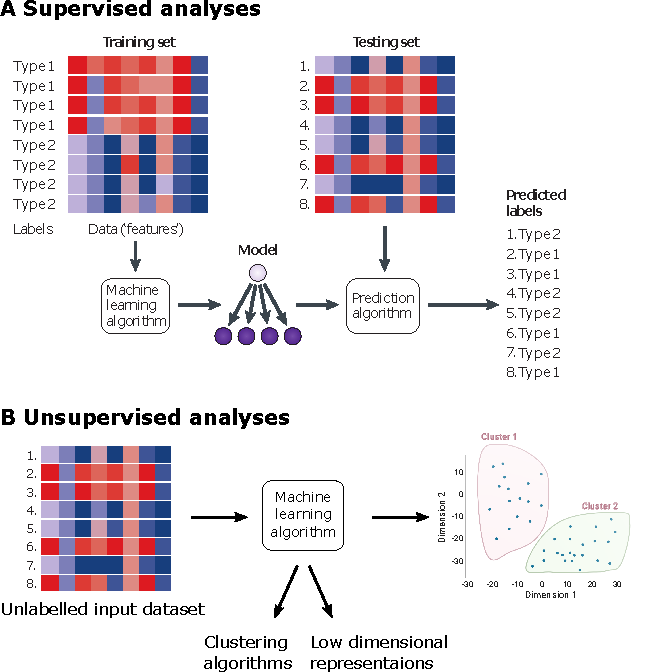
\includegraphics[width=1\textwidth]{Figures/Intro/supervised_vs_unsupervised.pdf}
    \caption[Machine learning methods: supervised vs non-supervised methods.]{\textbf{Machine learning methods: supervised vs non-supervised methods.} A) Supervised methods: a model is trained on several variables, features, to recognize predefined labels. The trained model is then applied to an unlabelled dataset for prediction purposes. B) Unsupervised methods: a model learns structures underlying a dataset that has not been labelled. Those methods are divided into two main categories: clustering methods to identify subgroups of samples and dimensionality reduction methods to explore the data in lower dimensions and highlight specific structures. Figure adapted from \cite{Libbrecht2015}. }
    \label{fig:intro_supervisedVSunsupervised}
\end{figure}

\textbf{Supervised analyses}
\newline 

The goal of supervised methods is to predict the value of an outcome based on a set of features given as inputs. Depending on the type of outcome, supervised analyses can be further divided into two main categories: classification or regression problems. In classification problems, the outcome is categorical, \textit{e.g.} a binary variable distinguishing a diseased or healthy status or a multi-classes variable like cancer subtypes. In regression problems, the objective is to predict a continuous variable. Note that some regression models, like logistic regressions, where the outcome variable is discrete, can be used though to perform classification.  
The main steps of supervised analyses consist in: i) defining the labels of each sample in the dataset, ii) train the model to classify the samples in the correct category, and iii) use the generated model on a dataset containing independent and unknown instances (Figure \ref{fig:intro_supervisedVSunsupervised}A). %Firstly, each element of the dataset has to be labelled, \textit{i.e.} each element belong to a pre-defined category. A machine learning model is then used to learn, from a set of variables, called features, how to classify each element in the correct category.
Several types of supervised methods exist and have to be chosen with regard to the nature of the data. The simplest supervised models are regression models. While the most common regression algorithms model linear relationships, other methods like \gls{SVM} or neural networks can adapt to non-linear data. Another parameter that determines the type of methods to use is the data type; some methods deal only with numerical features while others like decision trees are more flexible. Figure \ref{fig:intro_randomforest} describes a method based on decision trees, the random forest algorithm. 

\begin{figure}[H]
    \centering
    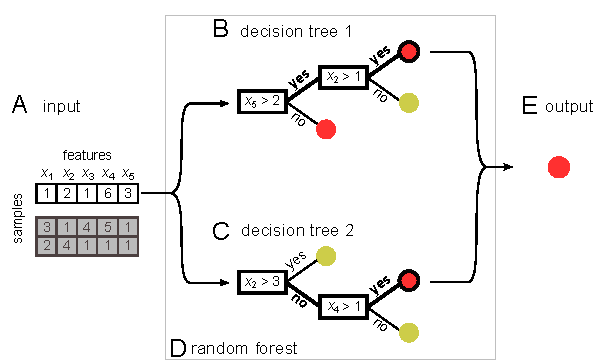
\includegraphics[width=0.8\textwidth]{Figures/Intro/random_forest.pdf}
    \caption[The random forest method]{\textbf{The random forest method.} Figure from \cite{Denisko2018}. A labelled dataset (A) is taken as input and processed by multiple decision trees (B and C) built using random selections of features and samples. The decision trees form a random forest (D). Each tree classifies the input samples and the votes given by the different trees are then combined to provide the final predictions. The label with the most votes being chosen (here red label). }
    \label{fig:intro_randomforest}
\end{figure}

%generalisation of the model
Regardless of the method used, the model and its results have to generalize to other datasets. In order to assess generalizability, the \gls{ML} algorithm has to be trained on a training dataset, and a testing dataset containing independent samples has to be used to validate the results. Two main errors underlying the generalization issue exist: bias and variance \cite{Domingos2012}. The first scenario occurs when the model is underfitting the data, \textit{i.e.} the model has a poor performance even on the training data for example because of a model that is not complex enough (See Figure \ref{fig:intro_biasVSvariance} left panel). When the model is underfitting the data, it is as well unable to generalize to other datasets. In the second case, when the number of features is too large or the number of samples small, the chances to encounter features that can perfectly discriminate two output categories or perfectly predict an outcome increase. The model, in that case, performs correctly on the training dataset but fails to generalize to other datasets and is qualified as high variance model. Such performance discrepancy indicates that the model overfits (See Figure \ref{fig:intro_biasVSvariance} right panel). Note that in high dimensional data, overfitting and data sparsity, resulting from the $n<<p$ problem mentioned at the beginning of this section, can be linked. Indeed, in such data, since the number of samples in the training dataset is fixed and limited, the entire input space is not covered. Thus the machine learning algorithm has not faced all possible configurations during the learning phase and the ability of the model to generalize can be diminished. 
\begin{figure}[H]
    \centering
    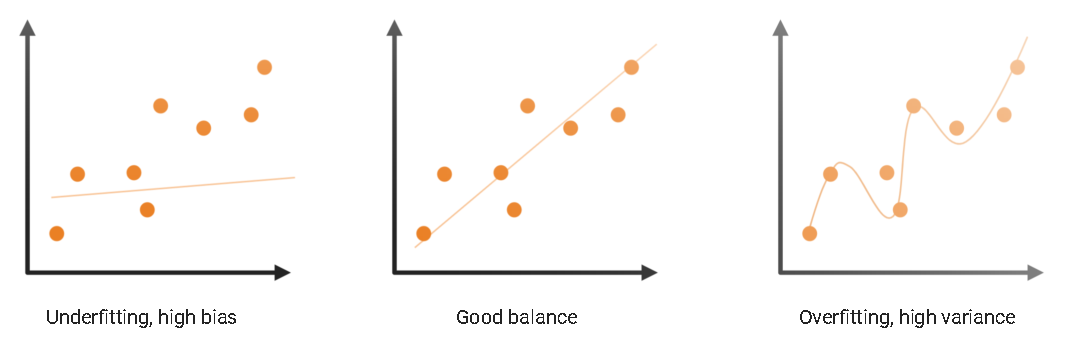
\includegraphics[width=0.8\textwidth]{Figures/Intro/overfitting.pdf}
    \caption[High bias and high variance models]{\textbf{High bias and high variance models.} Created with \href{https://biorender.com/}{BioRender.com}. }
    \label{fig:intro_biasVSvariance}
\end{figure}

One method that can be used to detect as well as overcome overfitting is cross-validation. The method consists in randomly splitting the dataset in $k$ folds and iteratively training the model on $k-1$ folds while reserving the remaining $k$th fold for testing (See Figure \ref{fig:intro_crossvalidation}). The overall performance of the model can be assessed by averaging the performances in the testing folds from each iteration. As a result, while none of the samples is used simultaneously in the training and testing group, the entire dataset is used for training as well as is used in the testing phase. Hence, cross-validation can also be beneficial in studies with low sample sizes. One extreme case of cross-validation is the leave-one-out analysis, where $k=1$. Each sample is set aside from the training set and predicted at each iteration. 
\begin{figure}[H]
    \centering
    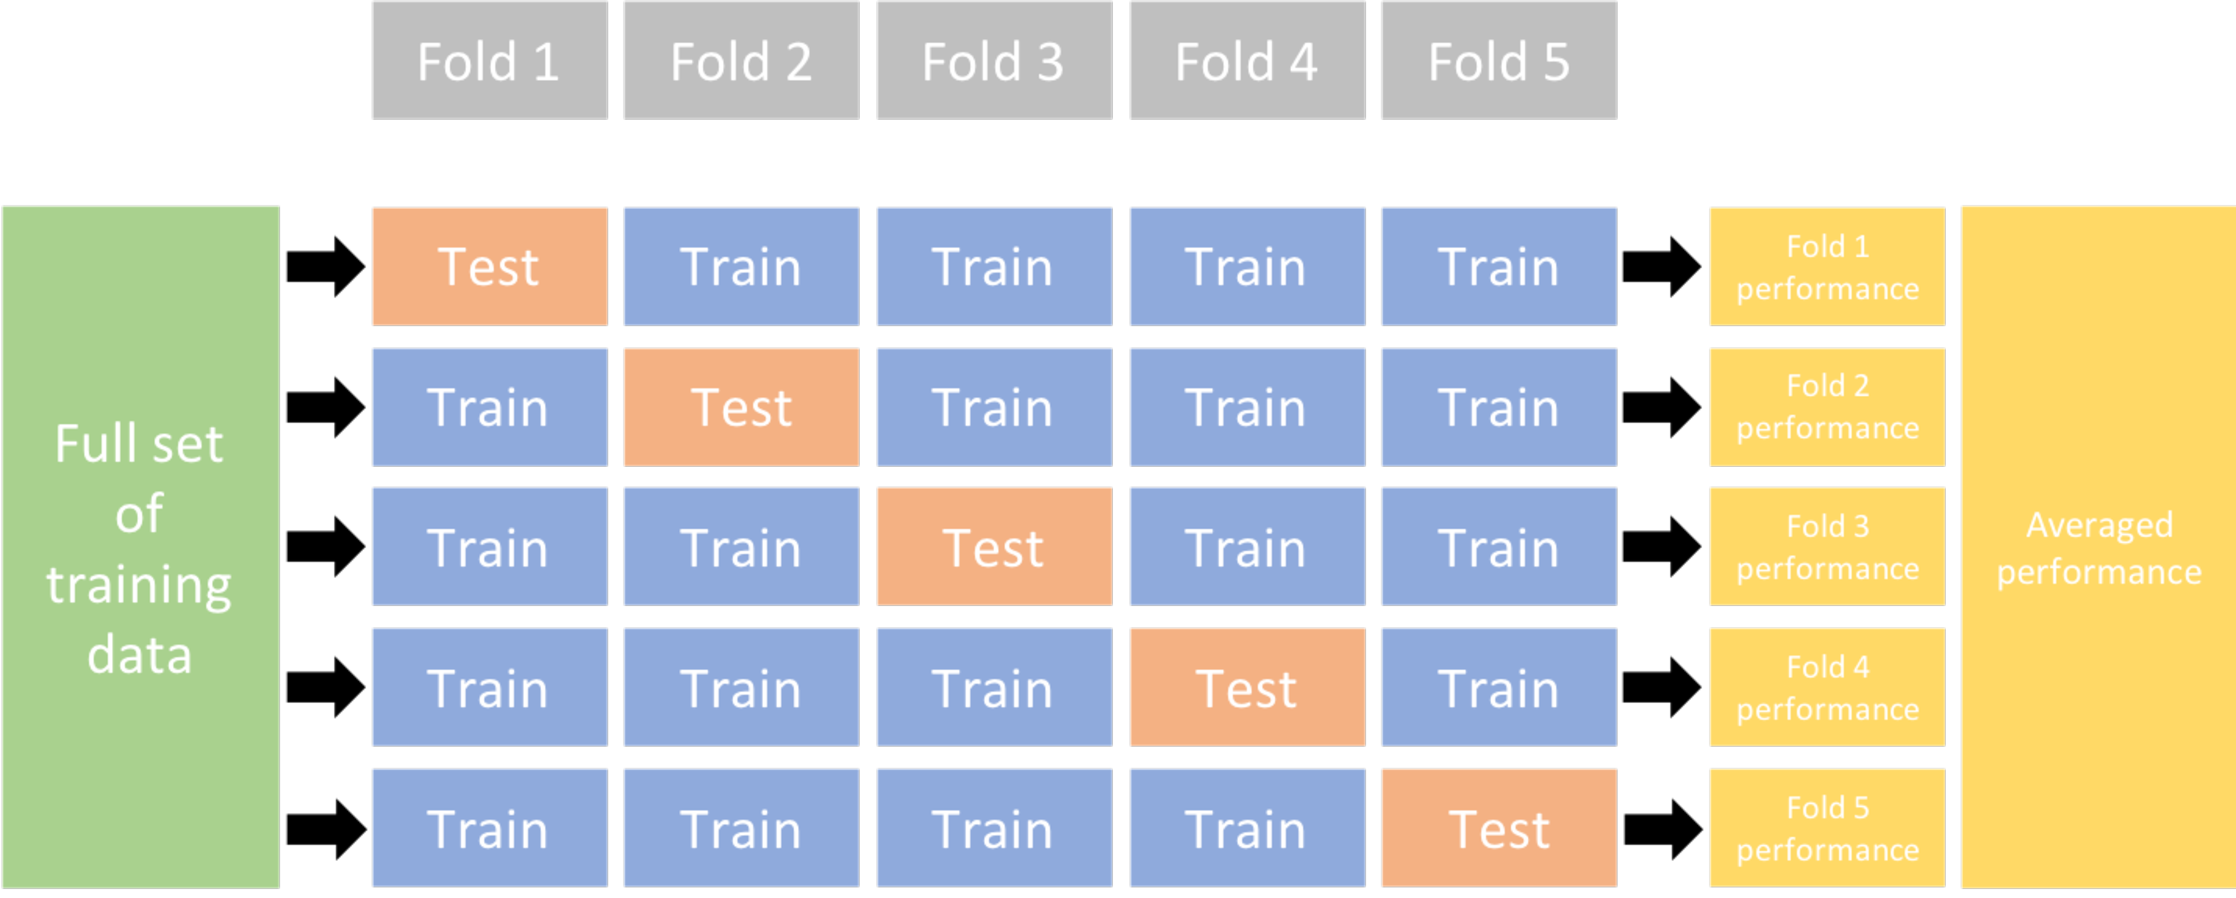
\includegraphics[width=0.9\textwidth]{Figures/Intro/cross_validation.pdf}
    \caption[$K$-fold cross-validation.]{\textbf{$K$-fold cross-validation.} Figure from \cite{BradleyBrandonGreenwell}. The figure illustrates 5-fold cross-validation. Five rounds are thus represented. In each of them, 4 folds are used to train the model and the model is tested on the remaining fold. The performances resulting from the test phase in each round are then averaged to estimate the overall performance of the model and its ability to generalize. }
    \label{fig:intro_crossvalidation}
\end{figure}

In addition, to find a compromise between bias and variance, parameter tuning and algorithm optimization might be required. Note that a third dataset, referred to as the validation dataset, can be introduced for the optimization step. In this setting, multiple models (\textit{e.g.} one algorithm with different sets of parameters or different algorithms) learn on the training set, and their performances are evaluated on the validation dataset. The model with the best performance can then be applied on the testing dataset.
\newline 

\textbf{Unsupervised analyses}
\newline 

Unsupervised algorithms are hypothesis-free methods and can be associated to exploratory analyses \cite{Oskolkov}. The goal of such methods is usually to identify and extract useful properties of the data \cite{Eraslan2019}. In contrast to the supervised methods, each element of the dataset is not labelled, no predefined groups are given to the algorithms. Thus, it is not possible to compare the algorithm output with a predefined truth and the data do not need to be split in training and testing datasets (Figure \ref{fig:intro_supervisedVSunsupervised}B). Since there is thus no feedback on the performance of the unsupervised model, often the validation of the results is required. 

As for the supervised analyses, there are several unsupervised algorithms. A commonly used category of unsupervised methods that can unveil structure in the data is the group of clustering algorithms (\textit{e.g.} $k$-means clustering, hierarchical clustering, density-based clustering). Those methods aim at grouping elements together based on common patterns observed in the set of features. In the field of cancer, clustering algorithms can be used, for example, to identify new subtypes of cancers based on molecular data. 
%Anomaly detection.
The second most commonly used unsupervised method is the group of dimensionality reduction methods. In the next paragraph, more details about such methods are provided.

%can generate hypotheses

\subsection{Dimensionality reduction methods}

The goal of \gls{DR} methods is to transform a high dimensional dataset into a low dimensional representation of the data while preserving as much as possible its initial structure. More specifically, if three clusters exist in the studied dataset, a lower dimensional representation of the same data should also reveal the initial three clusters. \gls{DR} methods are part of the feature extraction techniques which aim at finding latent structures in the data. Those methods allow to summarize and transform a large number of features in a smaller number of variables, which mitigates the curse of dimensionality and is valuable for data visualization. Note that these methods are different from feature selection methods, which make a selection of the most important features in the initial dataset \cite{Hastie2017}. Mainly two families of \gls{DR} methods exist: matrix factorization methods (\textit{e.g.} PCA, PLS, ICA, NMF) or neighbour graphs approaches (\textit{e.g.} t-SNE and UMAP). \newline


\textbf{Matrix factorization methods examples} \newline

Omics datasets, after pre-processing, often result in data matrices. For example, in the case of \gls{RNA-Seq}, after aligning the reads to a reference genome (See Figure \ref{fig:intro_ngs}), reads counting is performed and generates a matrix in which rows represent the genes (the features) and columns the read counts for each sample (the observations).  Matrix factorization consists in decomposing an initial matrix in two smaller matrices (Figure \ref{fig:intro_MF}). This decomposition leads to the generation of new variables, in smaller numbers. %In their review from 2018, Stein-O’Brien \textit{et al.} called the resulting matrices the amplitude and the pattern matrices \cite{Stein-OBrien2018}.
%In each matrix factorization method uses a different optimisation criterion to define the latent variables.

\begin{figure}[H]
    \centering
    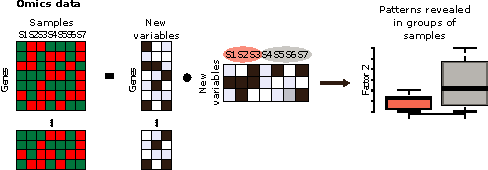
\includegraphics[width=0.9\textwidth]{Figures/Intro/MF_methods.pdf}
    \caption[Matrix factorization]{\textbf{Matrix factorization methods}. The input matrix is decomposed, under specific constraints, in two smaller matrices defined by new variables that can be used to reveal structures and patterns in the data.}
    \label{fig:intro_MF}
\end{figure}

A classical matrix factorization method is Principal Component Analysis (\gls{PCA}). The goal of \gls{PCA} is to project the data to a lower dimensional space while maximizing the variance in the data within this lower dimensional space. In \gls{PCA}, the new variables correspond to a linear combination of the initial features. The matrix factorization results in the loading and score matrices. In the first matrix, the columns correspond to the new variables, called principal components and the rows indicate the contribution of each feature to the latent variables. The principal components are orthogonal; they correspond to the directions of maximal variance and are ranked by the importance of variance explained, \textit{i.e.} the first principal component captures most of the variation in the dataset. The second matrix contains the coordinates of the samples in the projected space.
While \gls{PCA} maximizes the variance in the data, similar methods use other criteria. For example, \gls{ICA}, which is a method attempting at disentangling independent signals that are linearly mixed, maximizes the independence between the new variables. Other methods have in addition specific constraints \cite{Stein-Obrien2018}. \gls{NMF}, for example, enforces the decomposed matrices to be positive; this method has enabled the extraction of \textit{de novo} mutational signatures from whole genome sequencing data \cite{Alexandrov2013a}.
One limitation of those methods is that they are linear models. In the following paragraphs, two non-linear methods based on neighbour graphs are presented. \newline

\textbf{Neighbor graphs methods examples} \newline

The principle of \gls{DR} methods based on neighbor graphs models is to use neighbors distances and similarities to represent the structure of the data in high dimensions and then to embed this representation in a lower dimensional space. 

A method called \gls{t-SNE} \cite{VanDerMaaten2008} has been widely used in the past years to perform \gls{DR}. The \gls{t-SNE} method can be seen as a neighbor graph based algorithm \cite{McInnes2018} in a sense that similarity scores based on Euclidean distances between neighbors are computed to embed the high dimensional structure in a two-dimensional space. %The similarity between all the points is then calculated in the initial space and in the low dimensional space. 
Samples positions in the two-dimensional space are randomly initialized and are then moved iteratively so that the pair-wise samples similarities match the ones in the original space.  %Therefore, samples that are close to each others in the original space attracts each others.
\gls{t-SNE} has limitations though. Firstly, the method can be computationally intensive when applied to huge datasets. Also, the interpretation of the \gls{t-SNE} representation must be performed with caution. Indeed, the method retains local structures but has limited ability to maintain global structure \cite{McInnes2018}.  

Recently, a novel method called \gls{UMAP} \cite{McInnes2018} was developed and is more and more replacing the \gls{t-SNE} method. \gls{UMAP} is based on topological theory. The algorithm builds what is called a simplicial complex which is a representation of the data as a weighted graph (See Figure \ref{fig:intro_UMAP_topo}), the weights corresponding to the likelihood that there is a connection between two points \cite{McInnes_doc,AndyCoenen}.  
\begin{figure}[H]
    \centering
    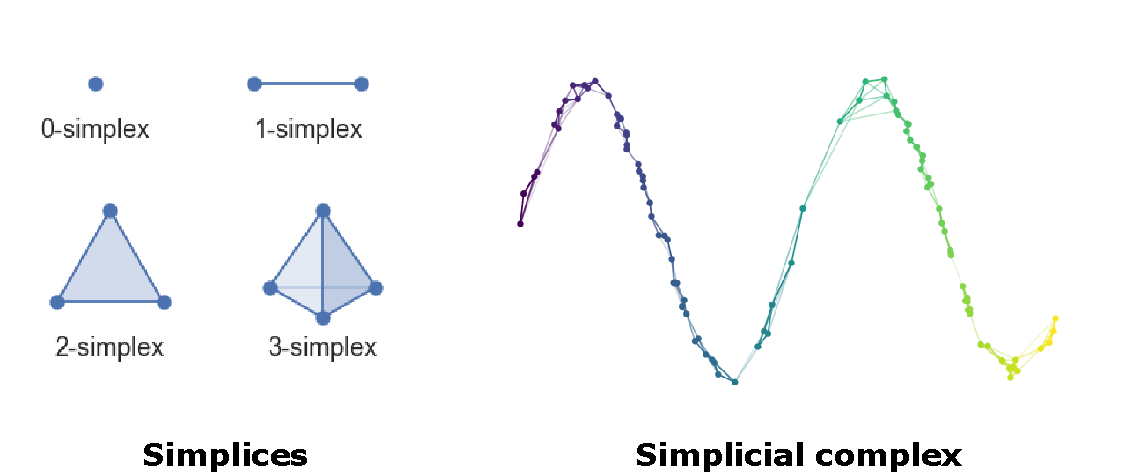
\includegraphics[width=0.9\textwidth]{Figures/Intro/simplicial_complex.pdf}
    \caption[UMAP topological representation]{\textbf{\gls{UMAP} topological representation}. A) The building blocks of a simplicial complex, the simplices. B) An example of a simplicial complex. Figures from \cite{McInnes_doc}.}
    \label{fig:intro_UMAP_topo}
\end{figure}
As mentioned at the beginning of Section \ref{Intro-method}, in high dimensional spaces data sparsity increases. To connect all the points in the simplicial complex, \gls{UMAP} varies the radius in which the search of neighbors is performed by fixing the number of neighbors to consider around each point \cite{McInnes_doc,AndyCoenen}. This number of neighbors influences how the data structure is preserved, low and high values favoring local and global structures, respectively. Once the graphical representation of the high dimensional data is constructed, a low dimensional representation of the data is optimized so that it is as close as possible to the high dimensional representation. % cross entropy
One of the advantages of \gls{UMAP} over \gls{t-SNE} is that the method better maintains the global structure of the data. Also, \gls{UMAP} is computationally more efficient \cite{McInnes2018}. Note that \gls{UMAP} can be applied on a lower dimensional dataset resulting, for example, from a \gls{DR} method like \gls{PCA}. 

% To connect each point to its closest neighbors, a radius is defined around each point and the points overlapping this radius are connected to the initial point. (using euclidean distance by default). 

%t-Distributed Stochastic Neighbor Embedding (\gls{t-SNE}), random initialization.  Computation of the similarity scores in the high and in the low representations. One of the problem of \gls{t-SNE} is that it does not scale to very large datasets.Also, the global structure of the data is not preserved, so inter-cluster differences can not be interpreted. Performing clustering on the resulting representation would not make sense. 

%To summarize, overcome overfitting issues and Dimensionality reduction methods help for the visualisation of such datasets \cite{DeAnda-Jauregui2020}. 
%Tmap: https://link.springer.com/article/10.1186/s13321-020-0416-x?shared-article-renderer

\subsection{Multi-omics data integration} 

The methods previously described consider as input a single dataset. \gls{DR} methods processing multiple matrices also exist and can be used to integrate multi-omics datasets. Such integration raises, though, multiple challenges. Firstly, the data to integrate are heterogeneous. The nature of the collected data is different, hence their statistical properties can vary. Also, it can happen that all the omics datasets are not available for each sample included in the analysis for technical reasons or due to quality issues. Hence, distinct patterns of missing data can occur in each omic dataset. Besides, integrating multiple datasets amplifies the curse of dimensionality issues already encountered in each dataset individually.

In 2018, a method called \gls{MOFA} was developed to integrate multi-omics data while considering the previously mentioned challenges \cite{Argelaguet2018}. \gls{MOFA} is an unsupervised analysis based on matrix factorization (See Section \ref{Intro-method}), and can be seen as an extension of \gls{PCA} to multi-omics data, called modalities or also views. It is a factor analysis method which reduces the dimensions of the data to a smaller number of unobserved factors, called the latent factors. These factors differ from the \gls{PCA} components. The latter are linear combinations of the initial features, while in factor analyses the initial features are expressed as linear combinations of the latent factors, plus a residual noise term. To enable multi-omics data (modalities) integration, \gls{MOFA} supports different noise models depending on the nature of the data (continuous, counts or binary data). Based on this model, \gls{MOFA} identifies different sources of variations across multiple omics data. \gls{MOFA} presents though several limitations. The model does not capture non-linear relationships and assume features independence \cite{Argelaguet2018}. %Also, the method does not account for additional information on the samples structure (groups of samples, batches, samples conditions) \cite{Argelaguet2018,Argelaguet2020}. 
Also, additional features accounting for samples structure, such as groups of samples, batches or samples conditions, were not available in the initial version of \gls{MOFA} but have been recently introduced in a second version, \gls{MOFA}+ \cite{Argelaguet2020}. In this framework, the \gls{MOFA} dimensionality reduction is performed with regards to additional samples information (\textit{e.g.} batch or cluster information) to identify sources of variations shared between groups or exclusive to one of them.
%In this framework, the method can, on top of integrating multiple omics data, also consider multiple samples groups \cite{Argelaguet2020}.

%The latter limitation can be overcome by other integrative methods. 
Other integrative methods can take into consideration samples structure. For example, the \gls{PLS} method, which is a matrix factorization method, attempts to relate two matrices: a response matrix and a matrix gathering explanatory variables. The advantage of this method is that it ensures that the new variables resulting from the dimensionality reduction explain the response data.
In that sense, the \gls{PLS} method can be considered as a supervised \gls{DR} framework. While \gls{PCA} maximizes the variance of the components, \gls{PLS} maximizes the covariance between the latent components of the response and explanatory datasets \cite{Kim,Hastie2017}. 
%The partial least squares (\gls{PLS}) method. 
When the response data is a categorical variable, a variant of \gls{PLS} called \gls{PLS-DA} can be used to perform classification tasks, \textit{e.g.} samples groups prediction. 
In 2017, Lê Cao team published the mixOmics framework implementing multivariate analyses tools, including the \gls{PLS} methods previously described \cite{Rohart2017}. The mixOmics tools also include the \gls{DIABLO} method, which is a multivariate dimension reduction method that can be used for supervised multi-omics data integration \cite{Singh2019}. \gls{DIABLO} maximizes the correlation between the features of the different omics datasets, one of this dataset corresponding to the labelled samples. Hence, the method extracts what the authors call multi-omics signatures that are discriminant and can be used for prediction in a supervised framework.  %However the method require parameter tuning lack from sparsity, see arguments from \cite{Argelaguet2018}





%----------------------------------------------------------------------------------------
%	BIBLIOGRAPHY
%----------------------------------------------------------------------------------------

\printbibliography[heading=bibintoc]

%----------------------------------------------------------------------------------------
%	ABBREVIATIONS
%----------------------------------------------------------------------------------------
%\printnomenclature
\newpage
\printglossaries
\addcontentsline{toc}{chapter}{Acronyms}



%\end{comment}
%----------------------------------------------------------------------------------------

\end{document}  
